????




%Nous allons commencer par trouver un moyen de mesurer l'aire d'un \ncycle\ $\setproba{L}$, si tant est que cela signifie quelque chose. 
%Il existe une notion d'aire algébrique d'un \ncycle\ qui s'appuie sur le déterminant: si $\setproba{L} = A_1 A_2 \cdots A_n$, alors l'aire algébrique de $\setproba{L}$ est $\frac12 \dsum_{i=1}^{n} \det \big( \vect{\Omega A^{\,\prime}_i} , \vect{\Omega A^{\,\prime}_{i+1}} \big)$, une quantité indépendante du point $\Omega$ choisi.
%Quand \geogebra\ associe un nombre à un \ncycle\ $\setproba{L}$, il calcule la valeur absolue de son aire algébrique.
%Malheureusement, cette notion n'est pas la bonne candidate comme le montre l'exemple suivant,%
%\footnote{
%	Pour construire un tel exemple, il suffit de fabriquer un \ngone\ croisé en \og spirale \fg, et de penser au calcul de l'aire algébrique avec un point $\Omega$ au \og centre \fg\ de cette spirale, car $\frac12 \det \big( \vect{\Omega A_i} , \vect{\Omega A_{i+1}} \big)$ est l'aire algébrique du triangle $\Omega A_i A_{i+1}$.
%}
%mais l'aire algébrique sera néanmoins utile pour formuler un argument de continuité.
%
%%\newpage
%
%\begin{multicols}{2}
%	\centering\small\itshape
%
%	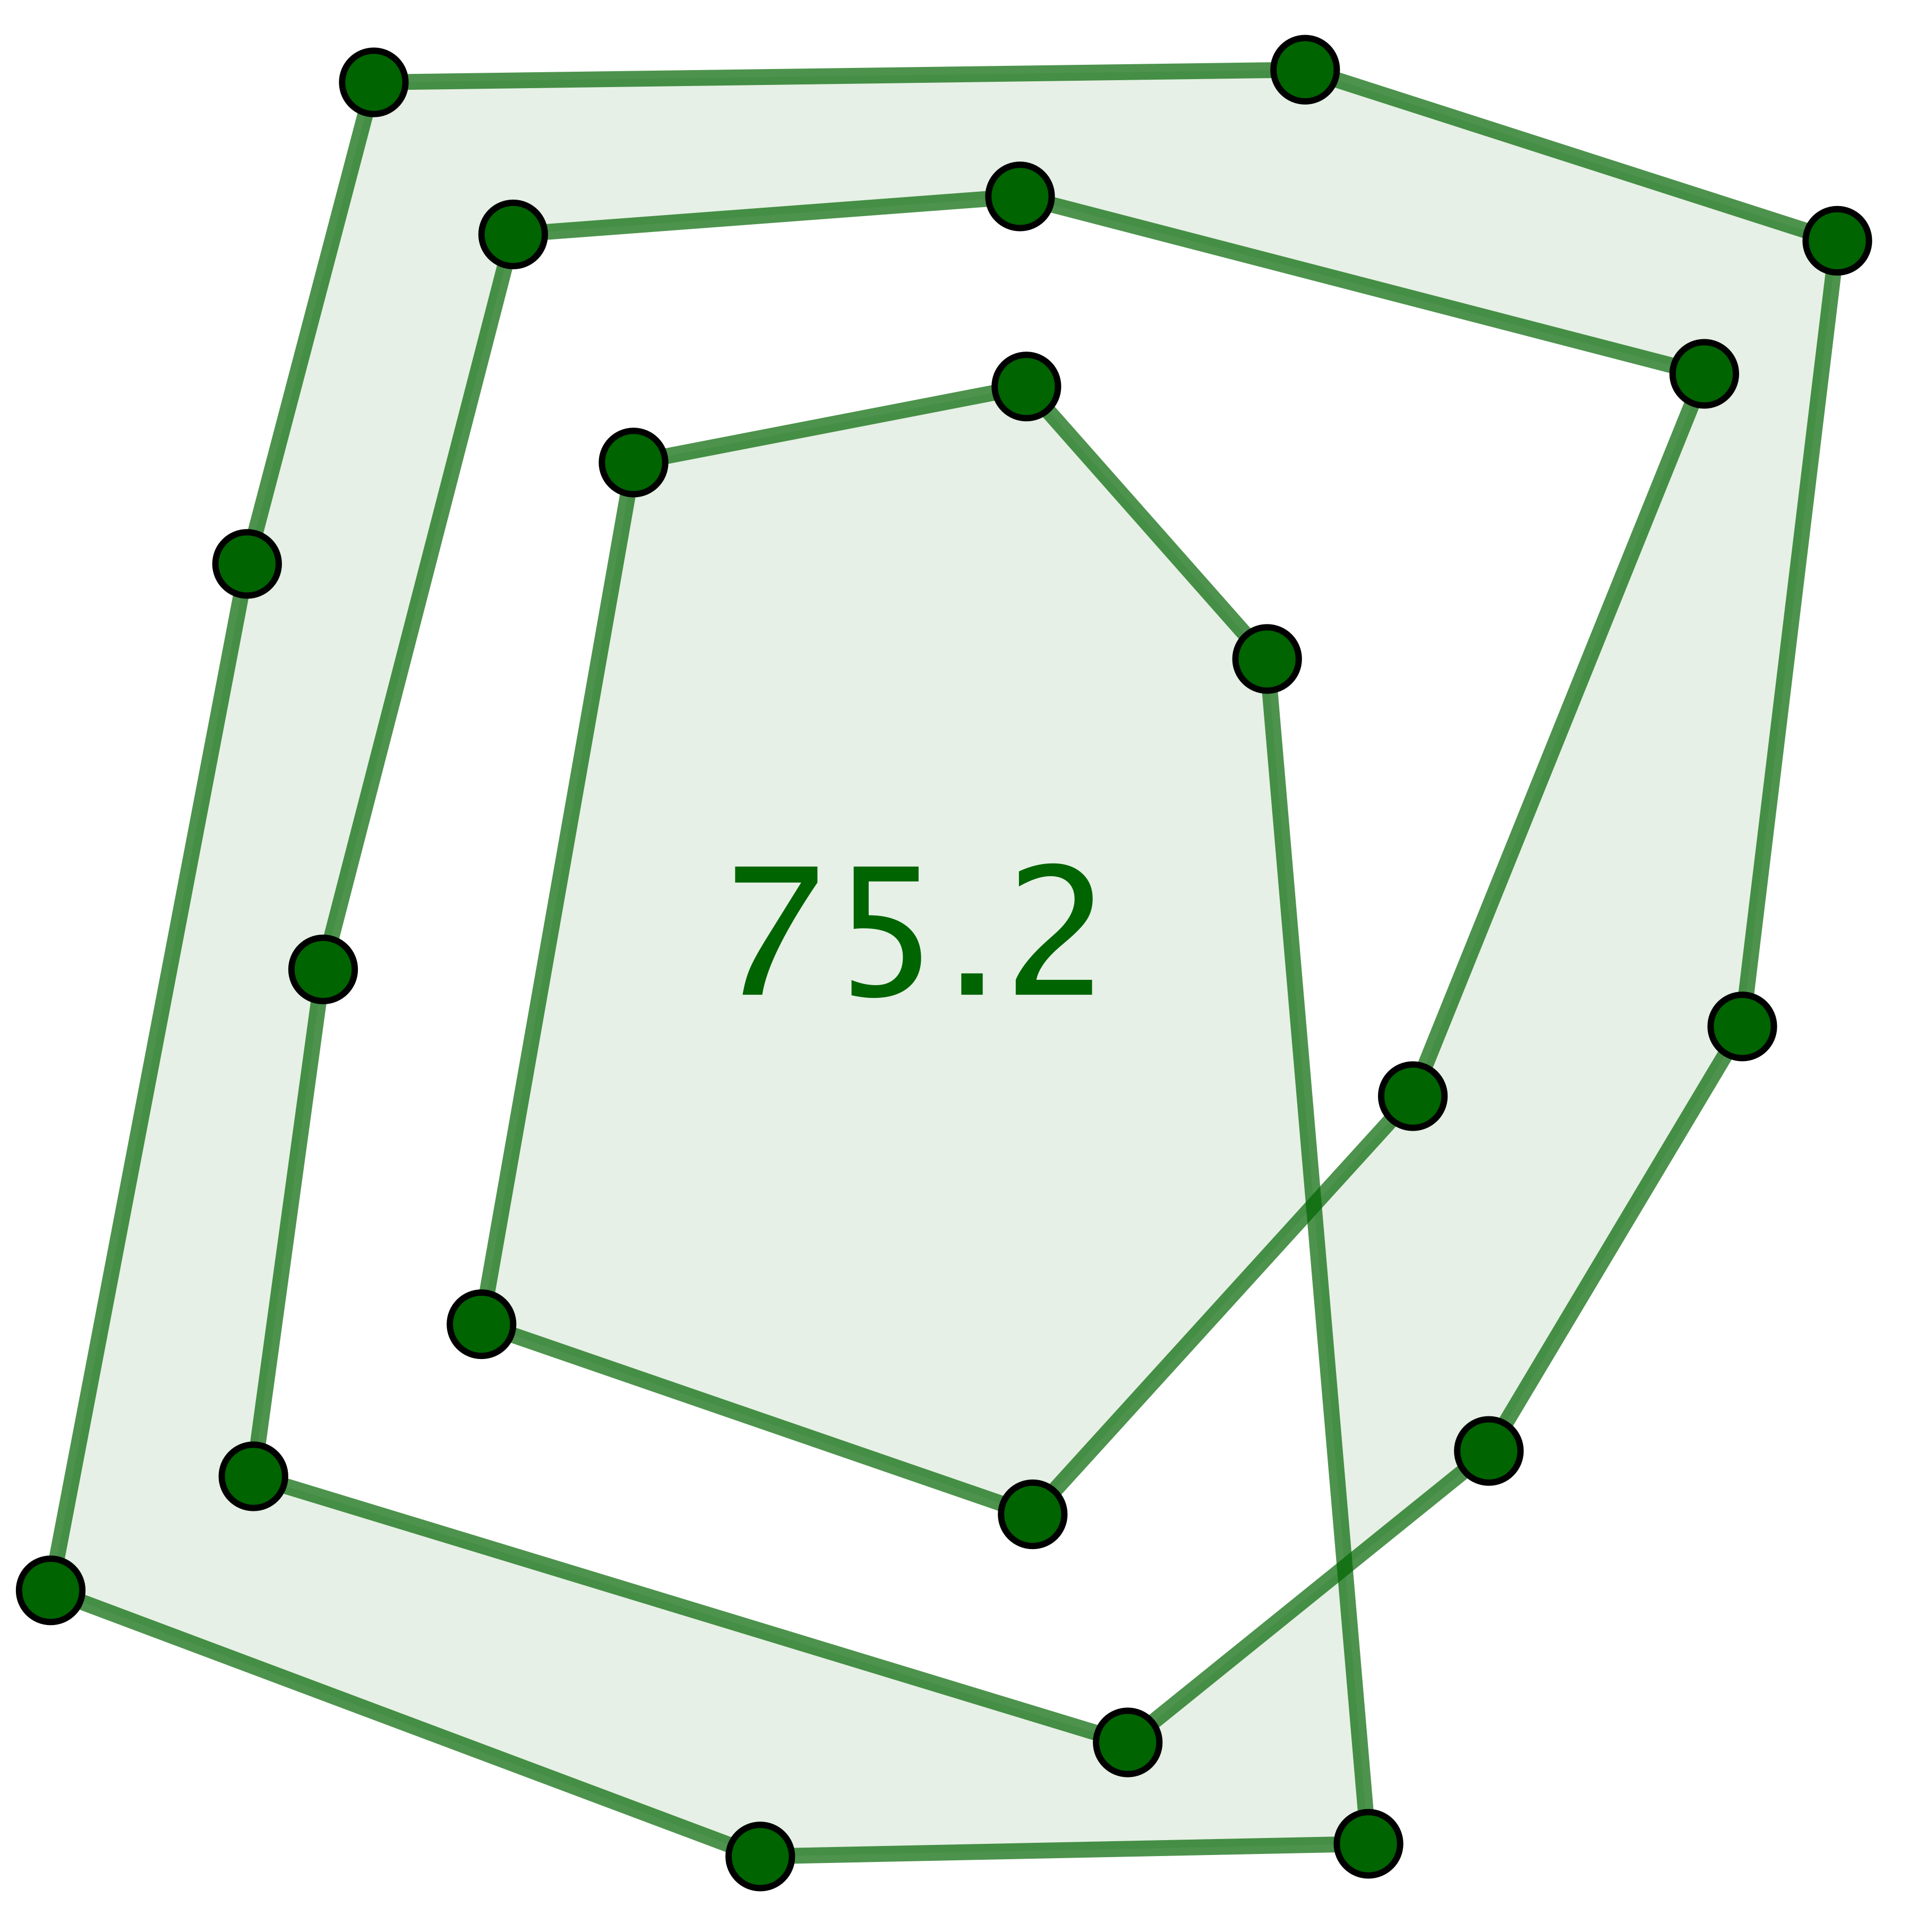
\includegraphics[scale=.35]{content/polygon/at-least-one/algarea-badforus-1.png}
%
%    \smallskip
%
%	Aire \og algébrique \fg\ d'un \ngone\ croisé $\setproba{P}$.
%
%	\columnbreak
%
%    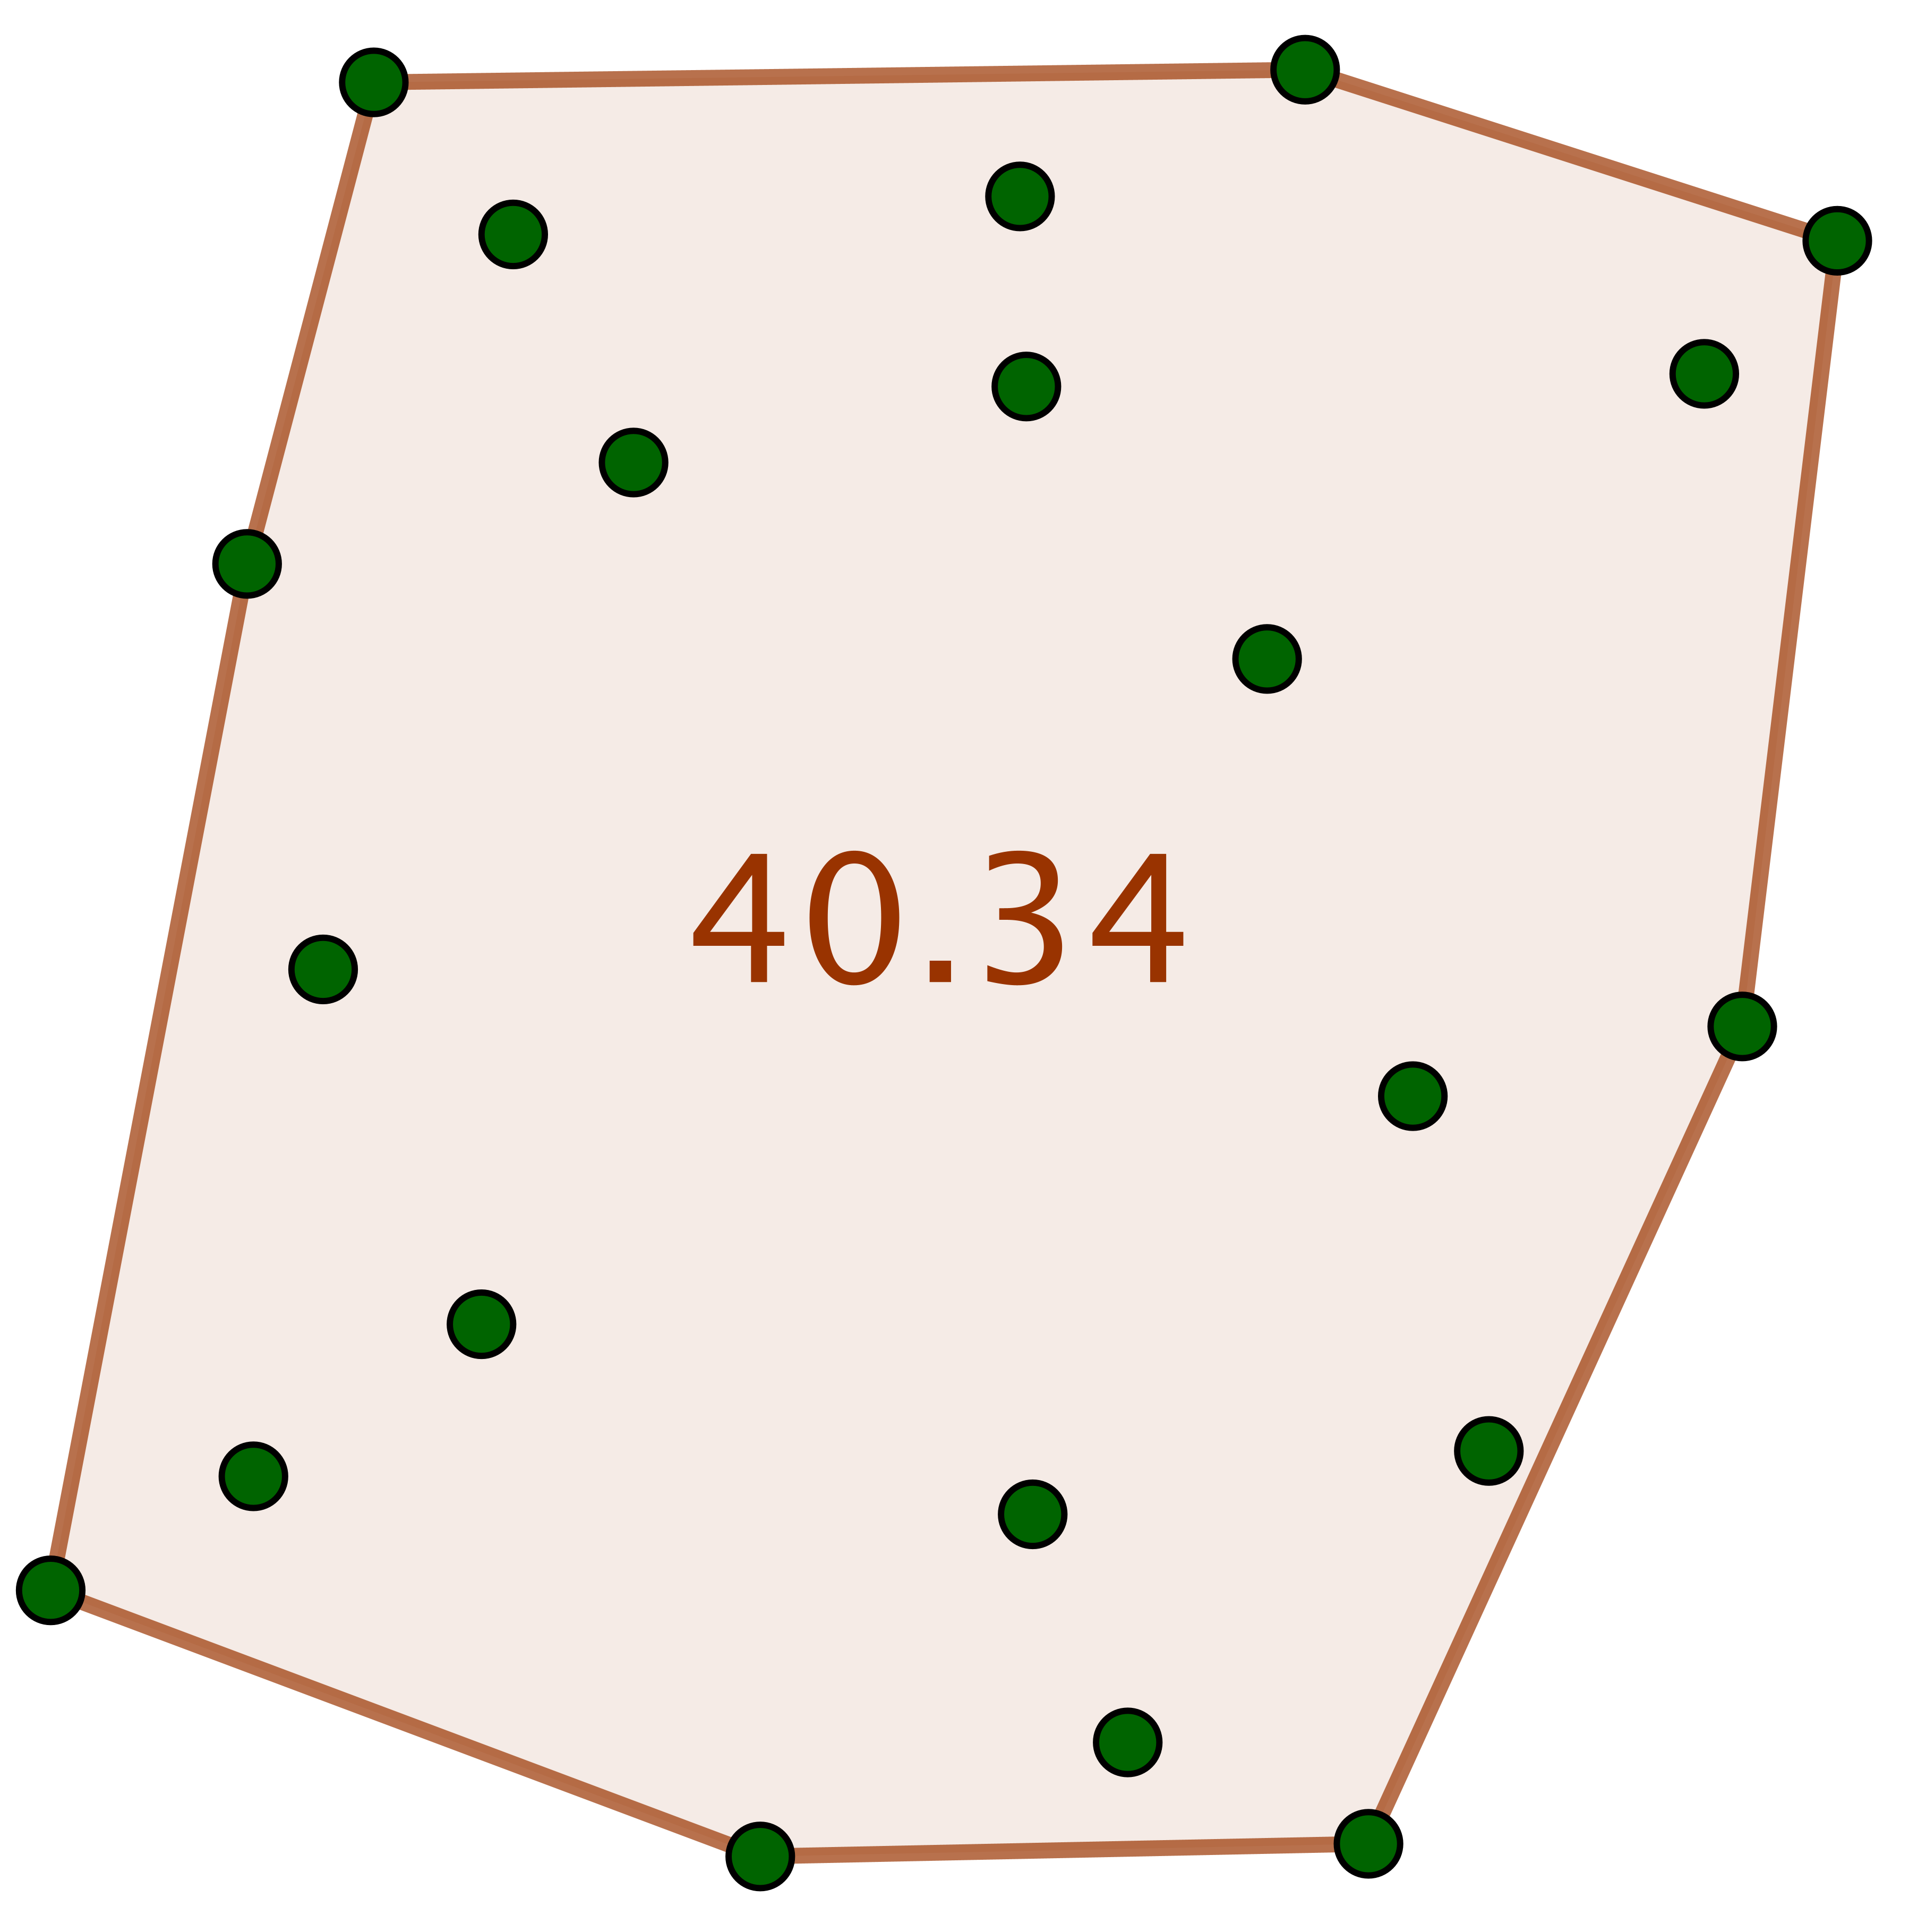
\includegraphics[scale=.35]{content/polygon/at-least-one/algarea-badforus-2.png}
%
%   	\smallskip
%
%	Aire de l'enveloppe convexe de $\setproba{P}$.
%\end{multicols}
%
%L'image de gauche nous donne la solution: il suffit de définir l'aire comme la somme des aires des \ngones\ coloriés par \geogebra. Sympa! Mais comment ce coloriage est-il fait? C'est un classique de l'informatique graphique, mais aussi un moyen de démontrer le faussement simple théorème de Jordan donnant l'intérieur et l'extérieur d'un \ngone. Voici comment cela fonctionne, sans chercher à démontrer les faits indiqués.
%%
%\begin{itemize}
%	\item Choisissons une direction orientée $\vect{\setgeo{d}}$ qui n'est parallèle avec aucun des côtés de $\setproba{L}$.
%
%	\item Considérons un point $M$ non situé sur le \ncycle\ $\setproba{L}$, et faisons partir une demi-droite $\setgeo{D}$ de $M$ suivant $\vect{\setgeo{d}}$.
%	On calcule alors $p(M)$ le nombre de points d'intersection de $\setgeo{D}$ avec le \ncycle\ $\setproba{L}$ en appliquant les règles suivantes.
%	%
%	\begin{enumerate}
%		\item Quand on rencontre un côté, mais pas un sommet, on ajoute $1$.
%
%		\item Quand on tombe sur un sommet, on ajoute $1$ si les voisins du sommet sont de part et d'autre de la demi-droite, et rien sinon.
%	\end{enumerate}
%
%	\item L'ensemble des points $M$ tels que $p(M)$ soit pair sera appelé la \og \emph{surface paire} \fg\ de $\setproba{L}$. 
%	On définit de même la \og \emph{surface impaire} \fg\ de $\setproba{L}$.
%	Une difficulté non négligeable reste à surmonter: s'assurer que le choix de la direction orientée ne modifie pas les surfaces paires et impaires obtenues.
%
%	\item La frontière de la surface impaire de $\setproba{L}$ est la réunion d'un nombre fini, éventuellement nul,%
%	\footnote{
%		Penser au cas d'un \ncycle\ dont tous les sommets sont alignés.
%	}
%	de \ngones\ d'intérieurs disjoints deux à deux.
%\end{itemize}
%
%
%\begin{center}
%	\small\itshape
%	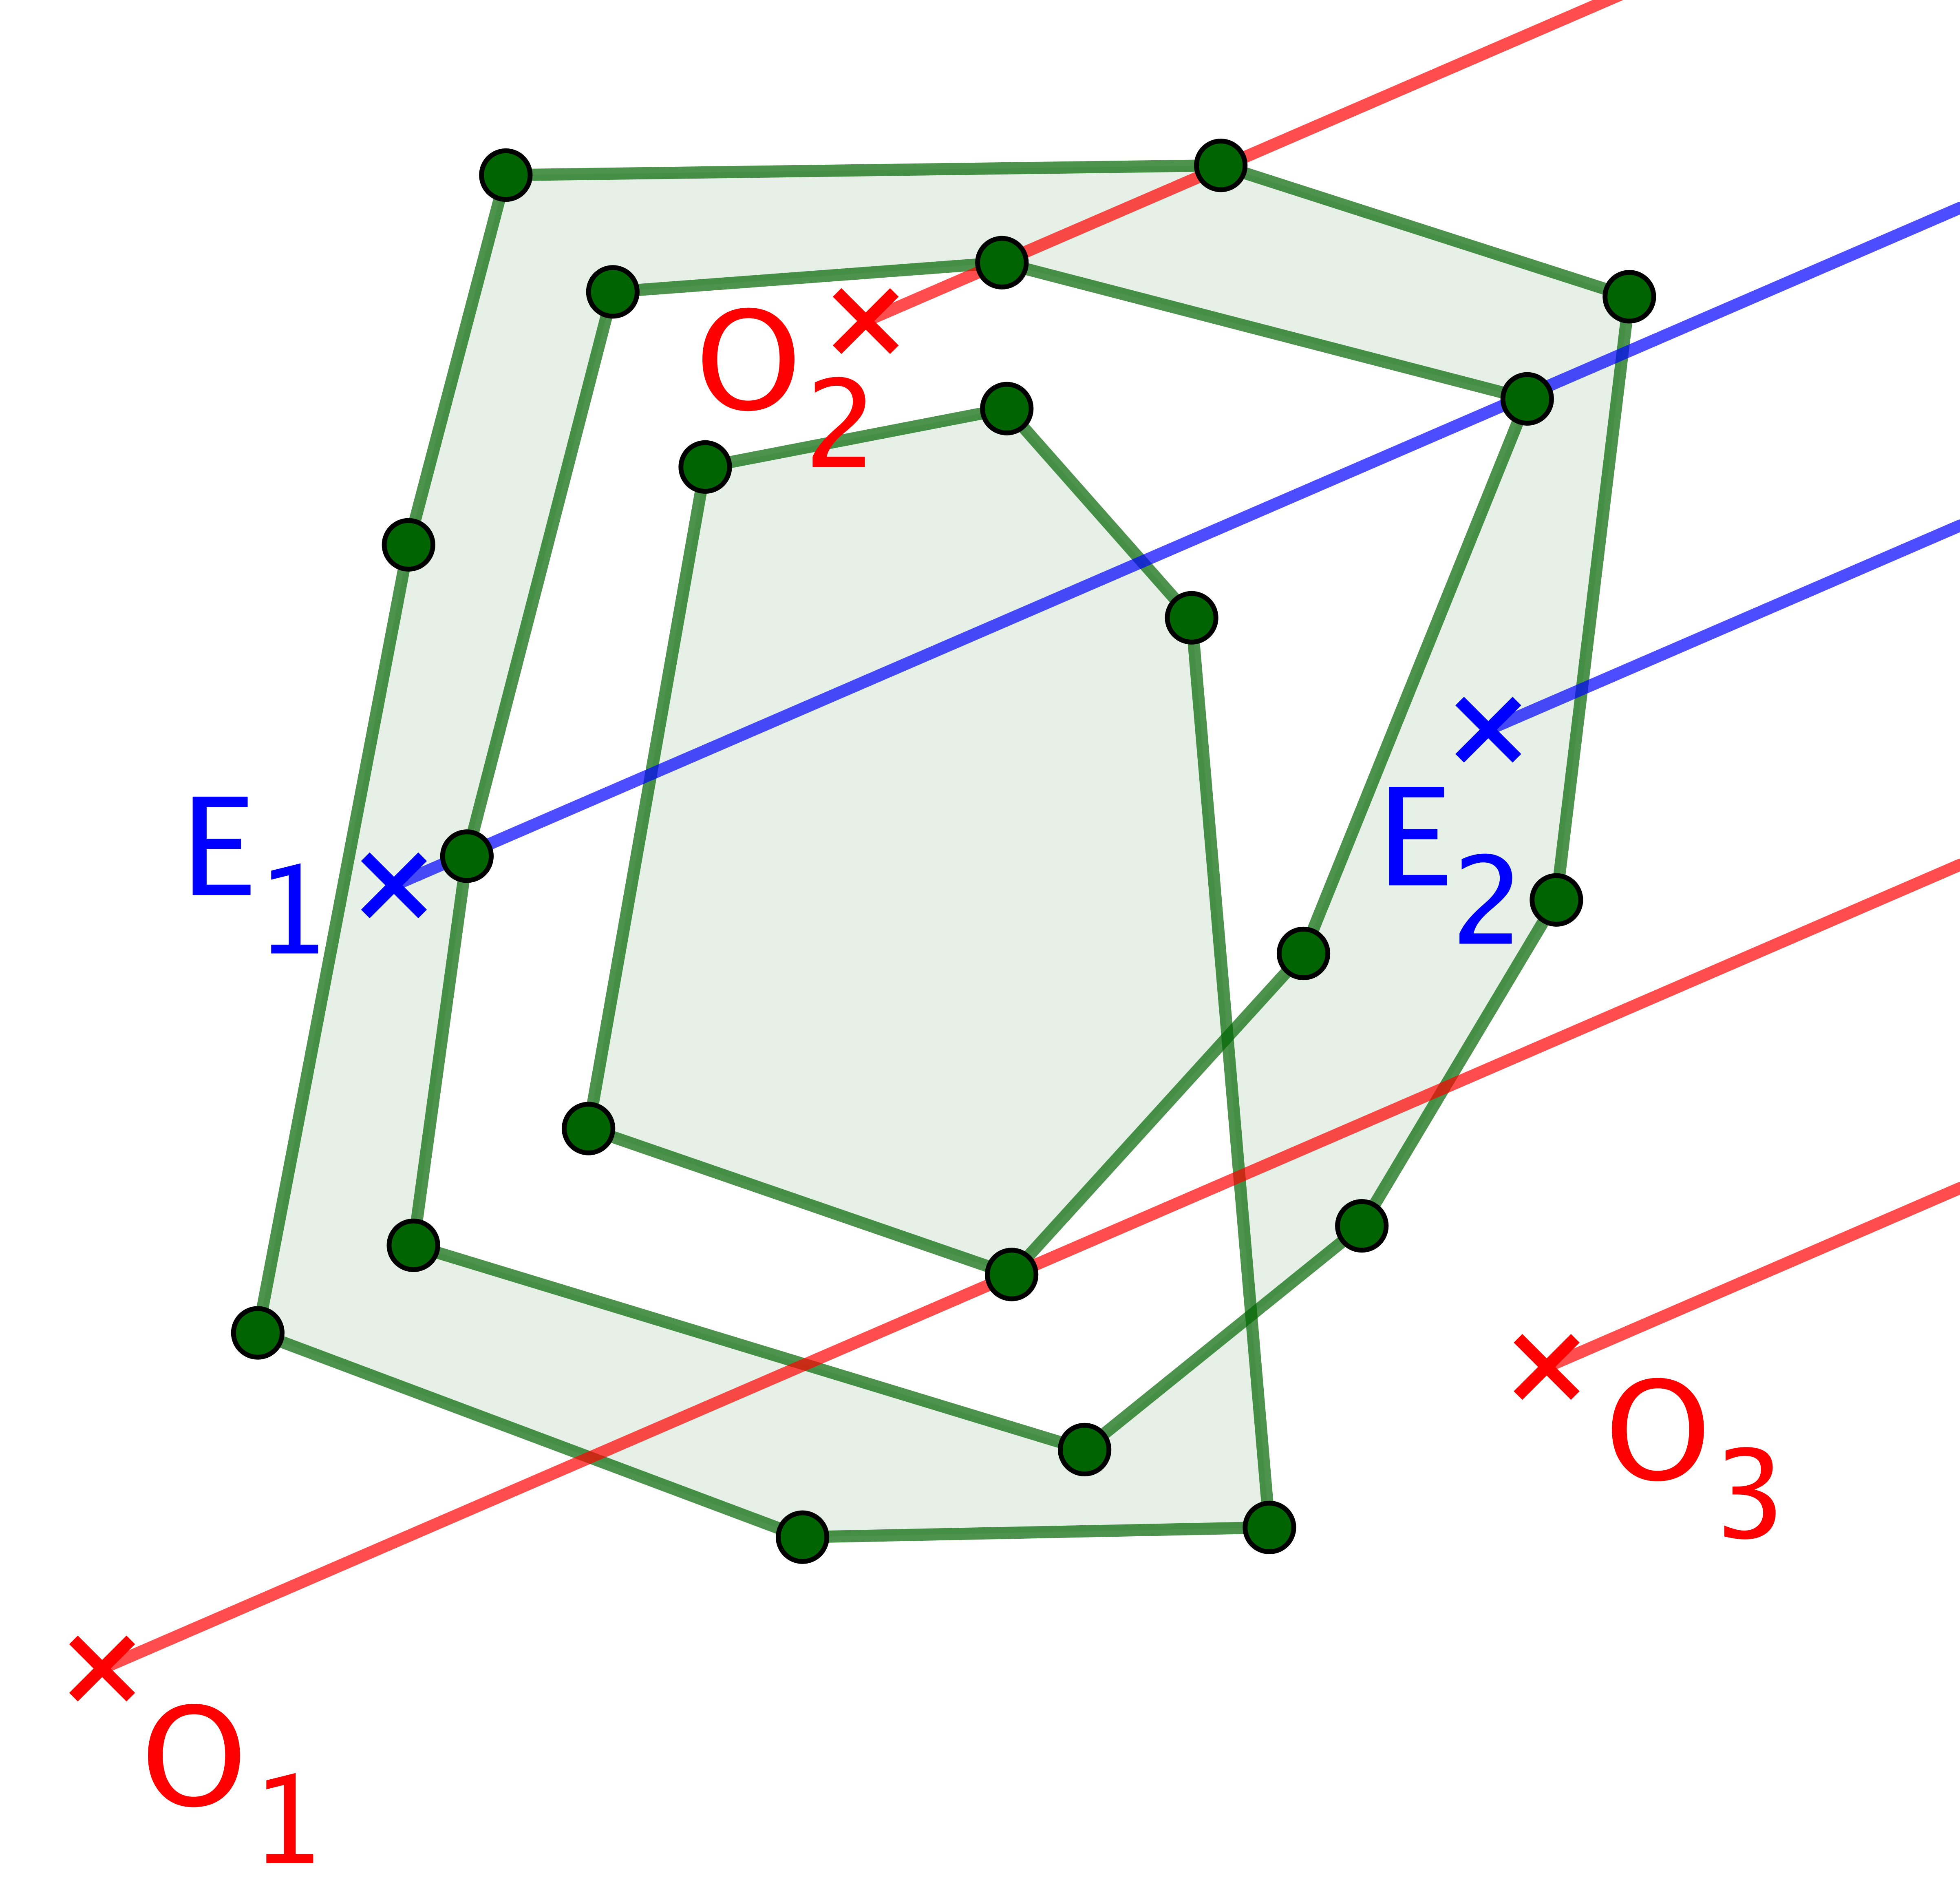
\includegraphics[scale=.3]{content/polygon/at-least-one/algarea-odd-even.png}
%	
%%	\smallskip
%	
%	Quelques calculs de $p(M)$:
%
%	\smallskip
%	
%	$p(E_1) = 5$,
%	$p(E_2) = 1$,
%%	
%%	\smallskip
%%	
%	$p(O_1) = 4$,
%	$p(O_2) = 2$ et
%	$p(O_3) = 0$.
%\end{center}
%
%
%\begin{defi} \label{garea-def}
%    Soit
%    $\setproba{L}$ un \ncycle\
%    ayant $\dcup_{i} \setproba{P}_i$ pour frontière de sa surface impaire, où les $\setproba{P}_i$, en nombre fini éventuellement nul, sont des \ngones\ d'intérieurs disjoints deux à deux.
%    La quantité $\garea{\setproba{L}} = \dsum_{i} \area{\setproba{P}_i}$ sera nommée \og \emph{aire généralisée} \fg\ du \ncycle\ $\setproba{L}$.%
%    \footnote{
%    	Rapellons qu'une somme de réels sur l'ensemble vide vaut zéro.
%    }
%\end{defi}
%
%
%% ----------------------- %
%
%
%\begin{fact}
%    Pour tout \ngone\ $\setproba{P}$, nous avons
%	$\garea{\setproba{P}} = \area{\setproba{P}}$.
%\end{fact}
%
%
%\begin{proof}
%	Immédiat.
%\end{proof}
%
%
%% ----------------------- %
%
%
%\begin{fact} \label{max-is-nconv}
%    Si un \ncycle\ $\setproba{L}$ de longueur non nulle n'est pas un \ngone\ convexe, alors il existe un \ngone\ convexe $\setproba{P}$ tel que
%	$\perim{\setproba{P}} = \perim{\setproba{L}}$
%	et
%	$\garea{\setproba{P}} > \garea{\setproba{L}}$.
%\end{fact}
%
%
%\begin{proof}
%	Commençons par le cas \og hyper-dégénéré \fg: si tous les sommets de $\setproba{L}$ sont alignés, son aire généralisée est nulle. Le triangle équilatéral de côté $\frac13 \perim{\setproba{L}}$ permet de conclure.
%	
%	Supposons maintenant que $\setproba{L}$ possède au moins trois sommets non alignés.
%	Notons $\setproba{C}$ l'enveloppe convexe de $\setproba{L}$ (nous savons donc que $\setproba{C}$ contient au moins un triangle).
%	
%	\begin{center}
%		\centering
%		\small\itshape
%		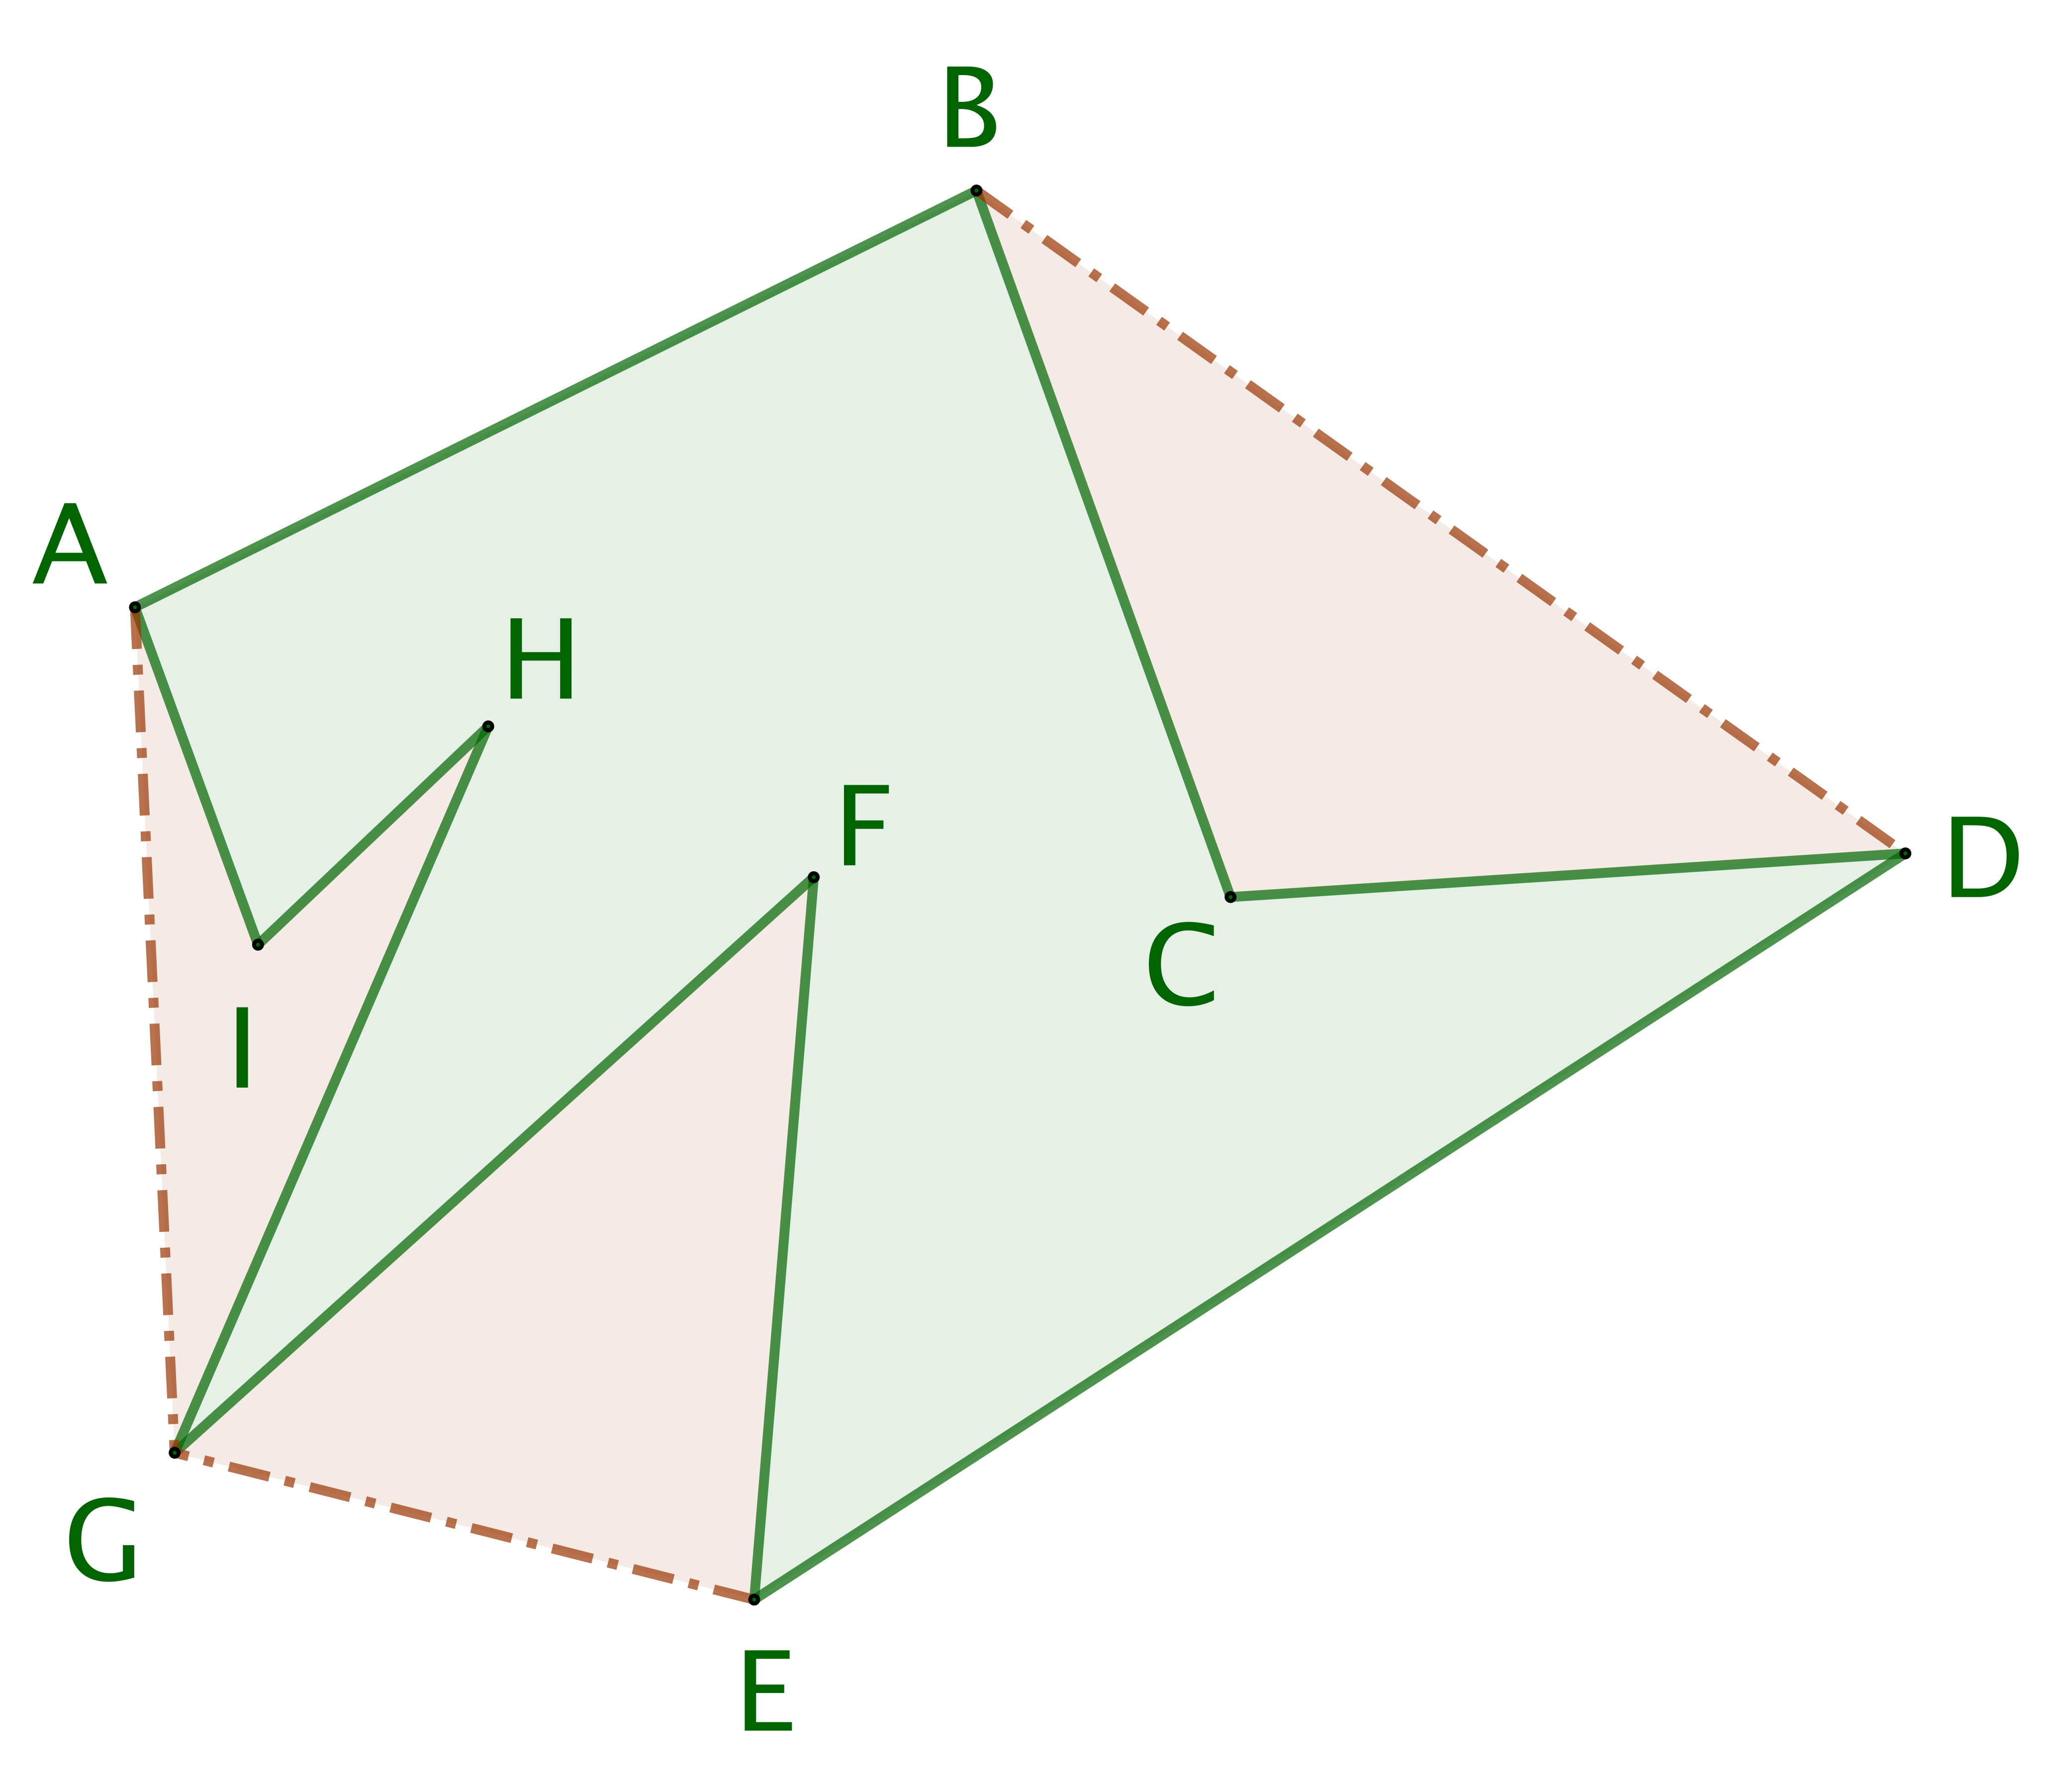
\includegraphics[scale=.45]{content/polygon/at-least-one/convex-hull.png}
%		
%		\smallskip
%		Exemple où $N = C$ et $O = B$.
%	\end{center}
%	
%		
%	Clairement, $\perim{\setproba{C}} < \perim{\setproba{L}}$.
%	Quant à $\garea{\setproba{C}} > \garea{\setproba{L}}$, c'est une conséquence directe de la définition de l'aire généralisé combinée au fait que $\setproba{L}$ ne soit pas un \ngone\ convexe.
%	Il reste un problème à gérer: $\setproba{C}$ est un \xgone{s} avec $s \leq n$. 
%	%
%	Une idée simple, formalisée après, est d'ajouter des sommets assez prêts des côtés de $\setproba{C}$ pour garder la convexité, une longueur strictement supérieure à $\perim{\setproba{L}}$, et une aire généralisée strictement plus grande que $\garea{\setproba{L}}$. Si c'est faisable, un agrandissement de rapport $r > 1$ donnera le \ngone\ $\setproba{P}$ cherché.
%	La figure suivante illustre cette idée.
%
%	\begin{center}
%		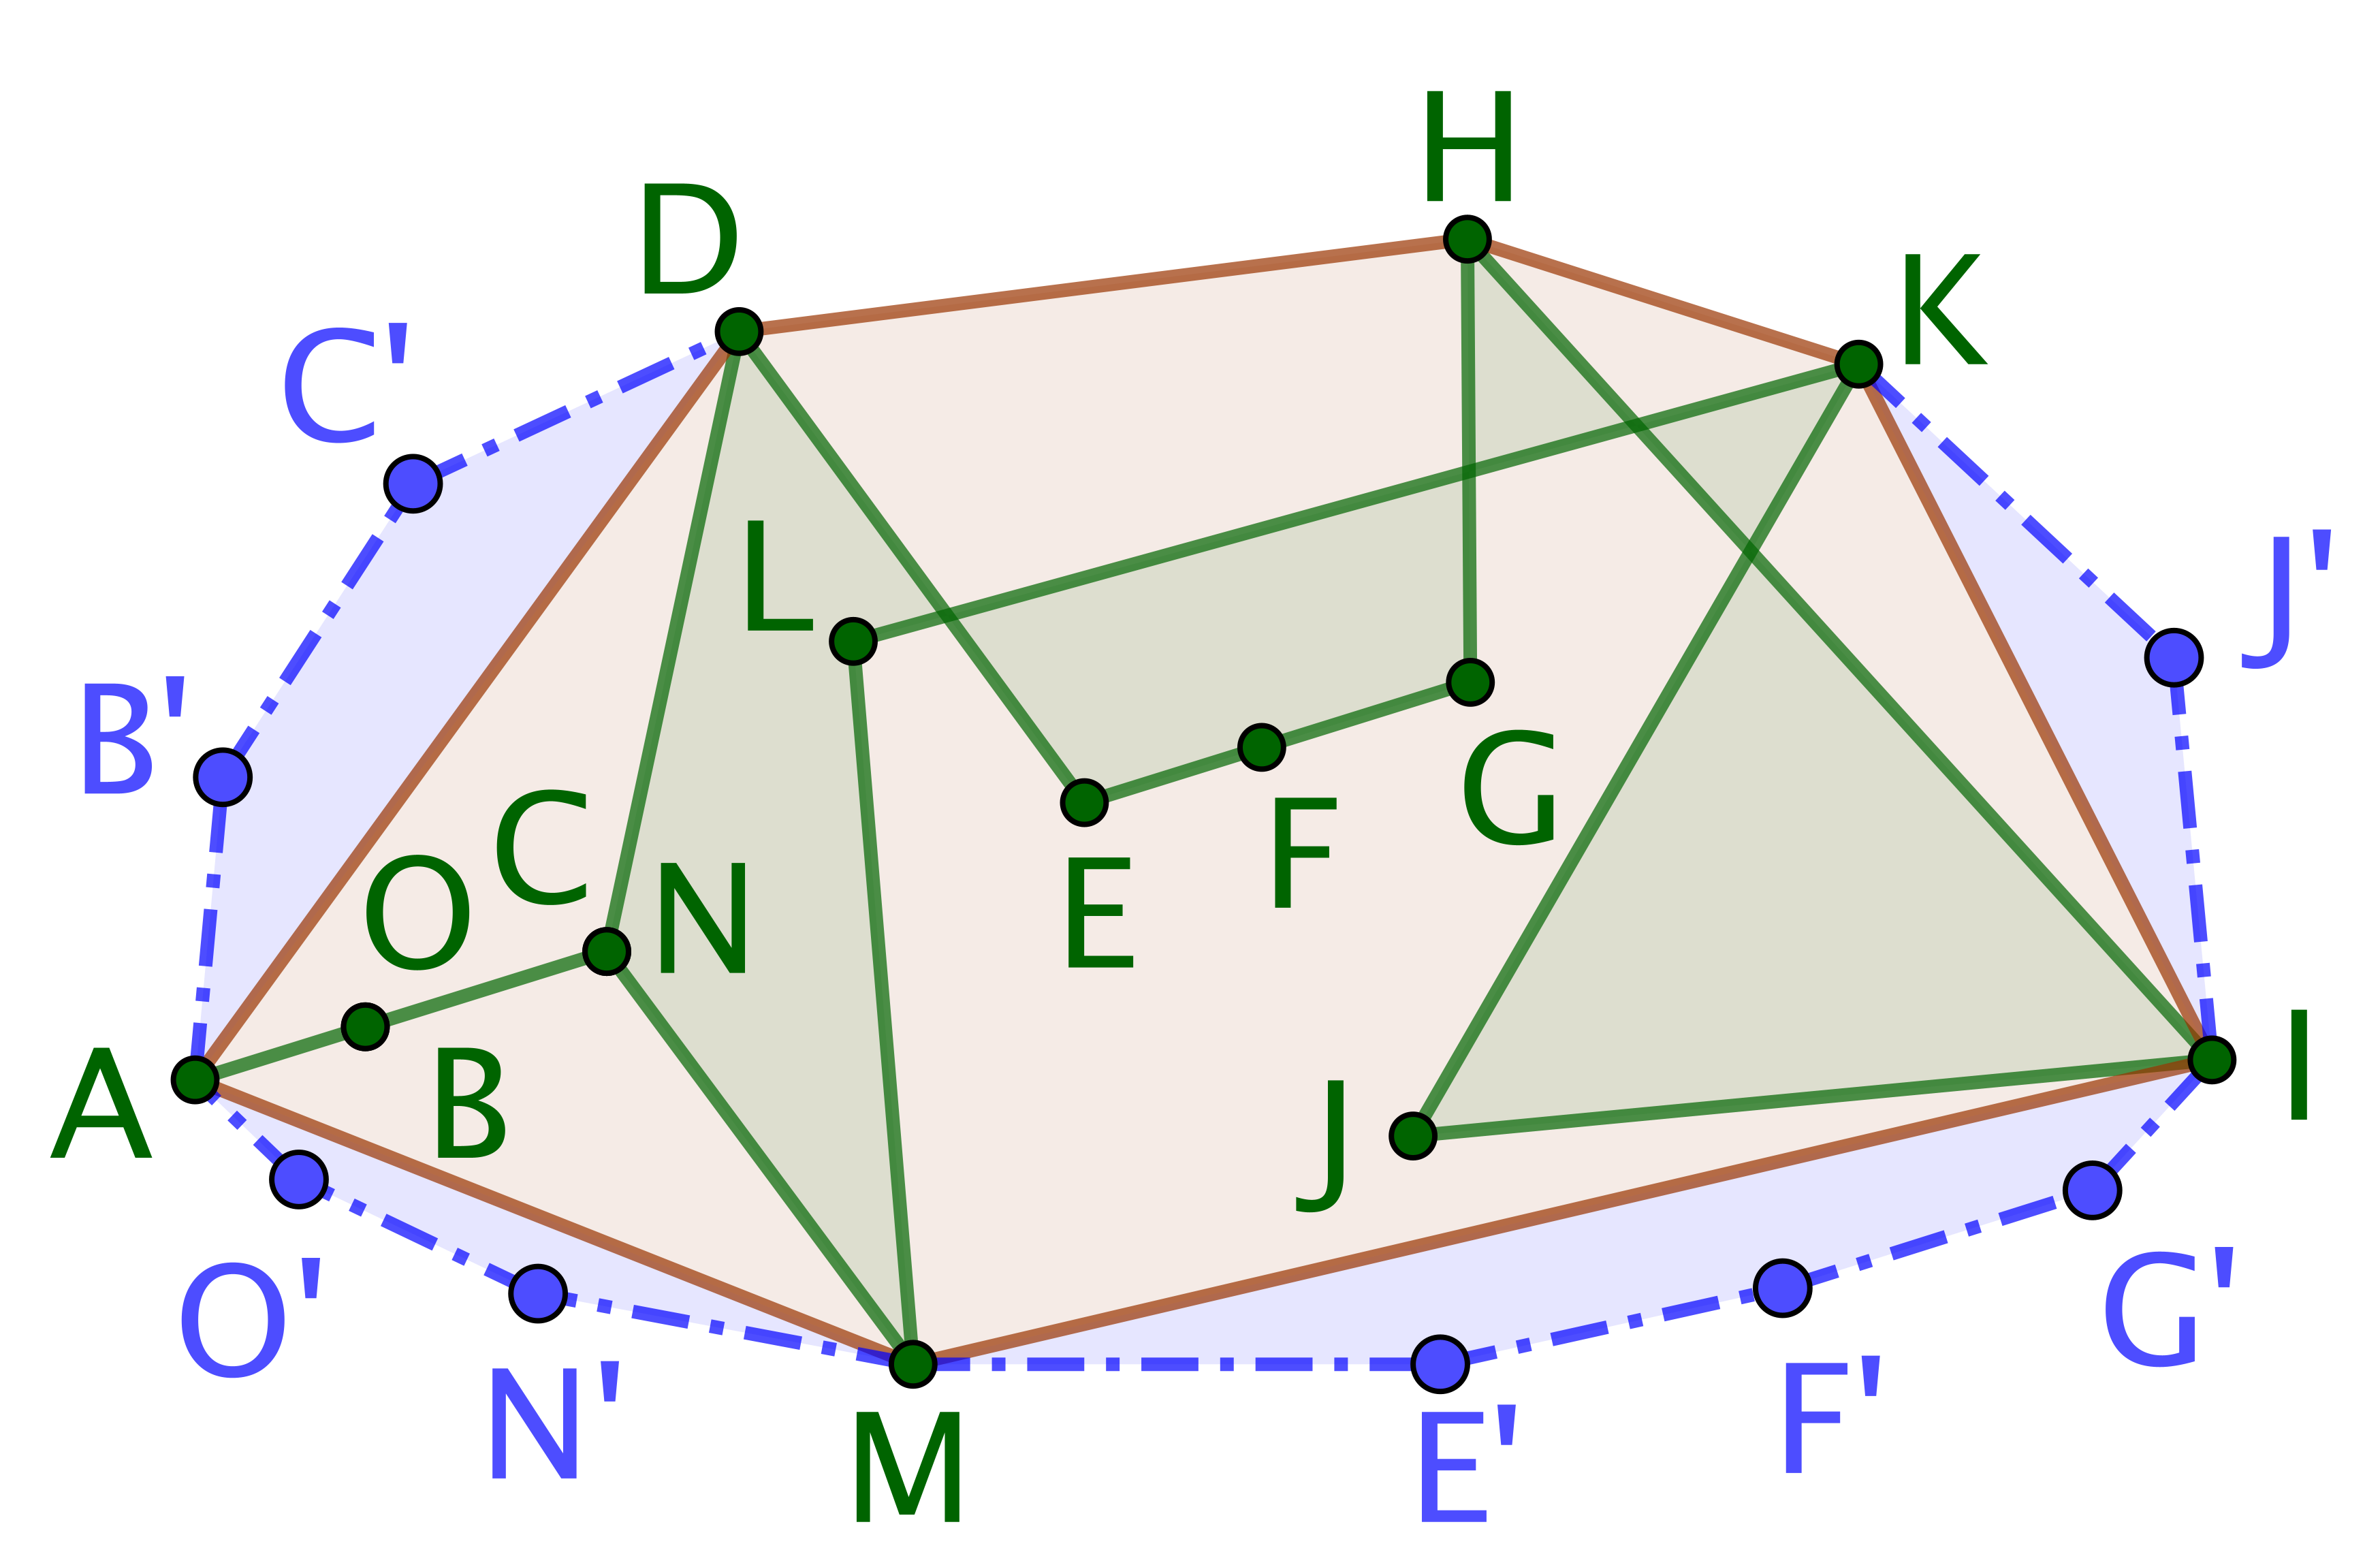
\includegraphics[scale=.45]{content/polygon/at-least-one/convex-hull-distortion.png}
%	\end{center}
%
%
%	$m = n - s$ compte les sommets manquants.
%	Si $m = 0$, il n'y a rien à faire.
%	Sinon, posons $\delta = \frac{\perim{\setproba{L}} - \perim{\setproba{C}}}{m}$.
%	%
%	\begin{enumerate}
%		\item \label{add-vertex-start}
%		Considérons $[AB]$ un côté quelconque de $\setproba{C}$.
%		Les droites portées par les côtés \og \emph{autour} \fg\ de $[AB]$ \og \emph{dessinent} \fg\ une région contenant toujours un triangle $ABC$ dont l'intérieur est à l'extérieur
%		\footnote{
%			C'est ce que l'on appelle de la \og \emph{low poetry} \fg\,.
%		}
%		de $\setproba{C}$ comme dans les deux cas ci-dessous.
%	%
%		\begin{multicols}{2}
%			\centering
%
%			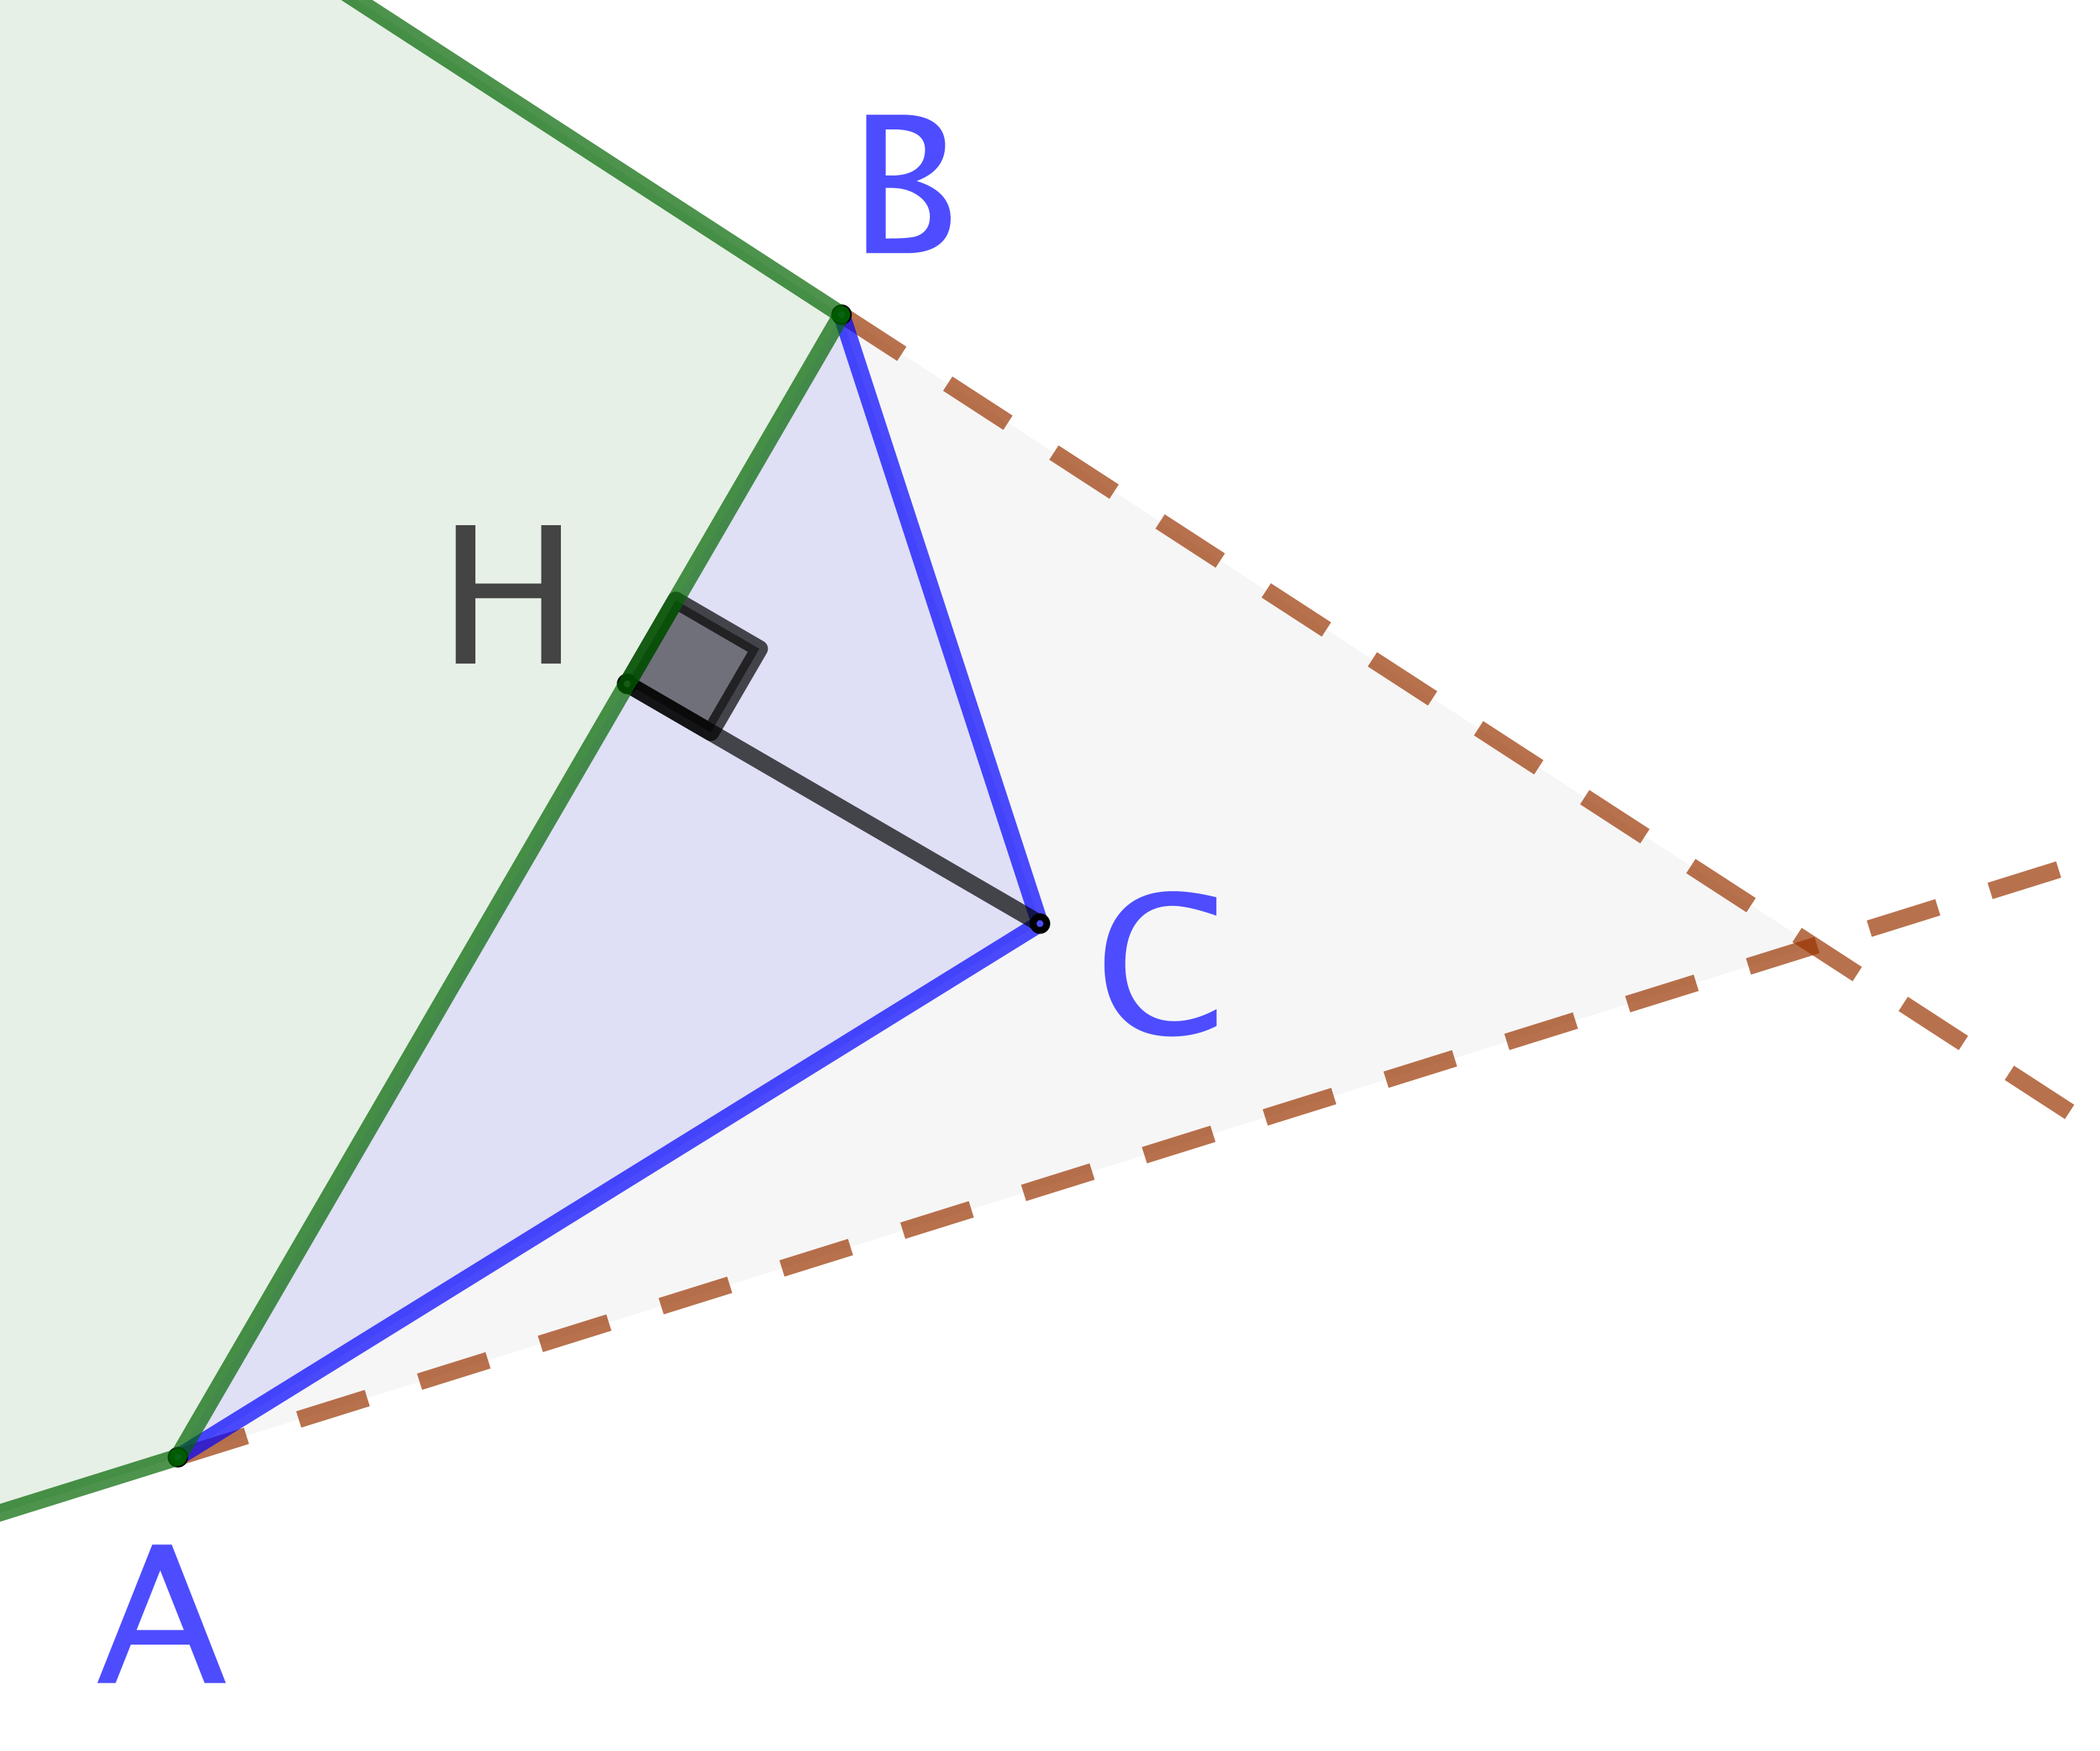
\includegraphics[scale=.35]{content/polygon/at-least-one/add-vertex-1.png}
%
%			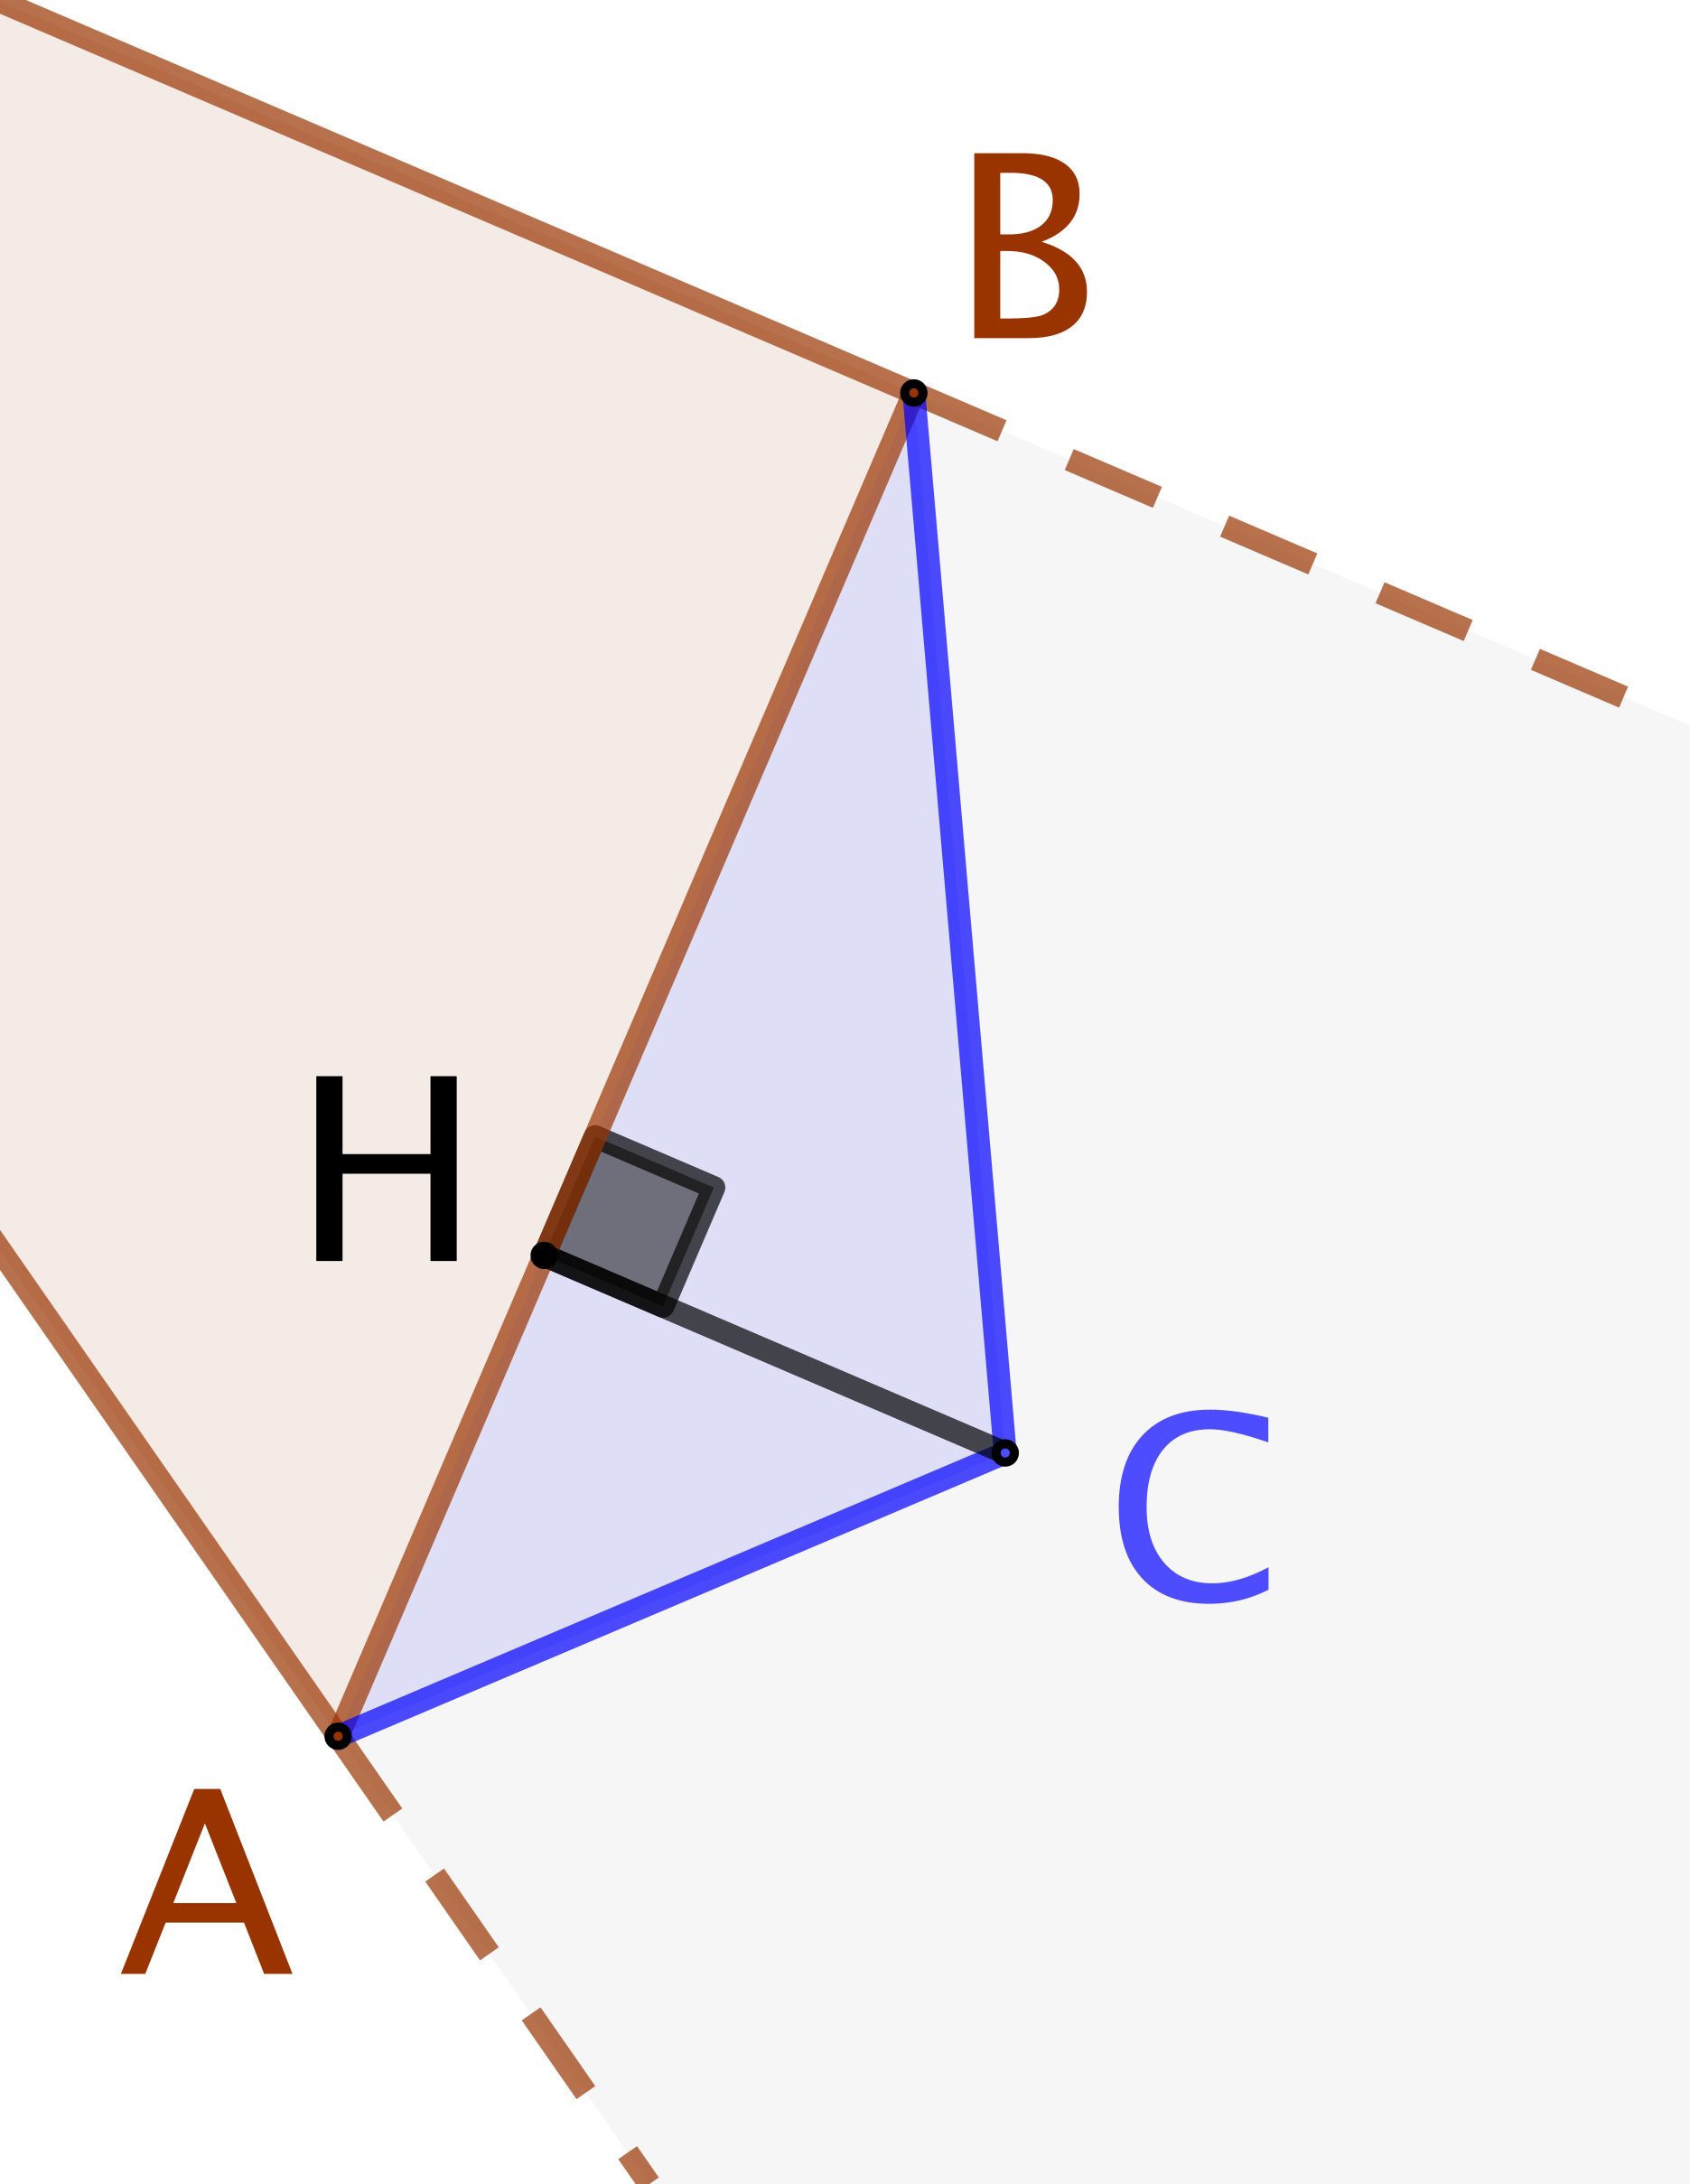
\includegraphics[scale=.35]{content/polygon/at-least-one/add-vertex-2.png}
%		\end{multicols}
%
%		\item Clairement, le polygone $\setproba{C}_+$ obtenu à partir de $\setproba{C}$ en remplaçant le côté $[AB]$ par les côtés $[AC]$ et $[CB]$ est un convexe avec un sommet de plus que $\setproba{C}$.
%
%		\item \label{add-vertex-end}
%		Comme $HC$ peut être rendu aussi proche de $0$ que souhaité, il est aisé de voir que l'on peut choisir cette distance de sorte que $AC + BC < AB + \delta$.
%		Dès lors, le périmètre de $\setproba{C}_+$ augmente inférieurement strictement à $\delta$ relativement à $\setproba{C}$.
%
%		\item En répétant $(m-1)$ fois les étapes \ref{add-vertex-start} à \ref{add-vertex-end}, nous obtenons un \ngone\ convexe $\setproba{P}$ tel que
%		$\garea{\setproba{P}} > \garea{\setproba{L}}$
%		et
%		$\perim{\setproba{P}} < \perim{\setproba{C}} + m \delta = \perim{\setproba{L}}$.
%	\end{enumerate}
%	
%	\null\vspace{-6ex}
%\end{proof}
%
%
%% ----------------------- %
%
%
%Enquêtons sur le calcul de l'aire d'un \ngone, afin de savoir si l'aire généralisée est \og continue \fg. 
%Comme $ABC$ est d'aire algébrique $\frac12 \det \big( \vect{AB} , \vect{AC} \big)$, avec $\area{ABC} = \frac12 \abs{ \det \big( \vect{AB} , \vect{AC} \big) }$, nous allons travailler avec des triangles comme dans l'exemple suivant.
%
%
%\begin{multicols}{2}
%	\small\itshape
%    \begin{center}
%		Calcul direct à la main.
%
%		\smallskip
%
%        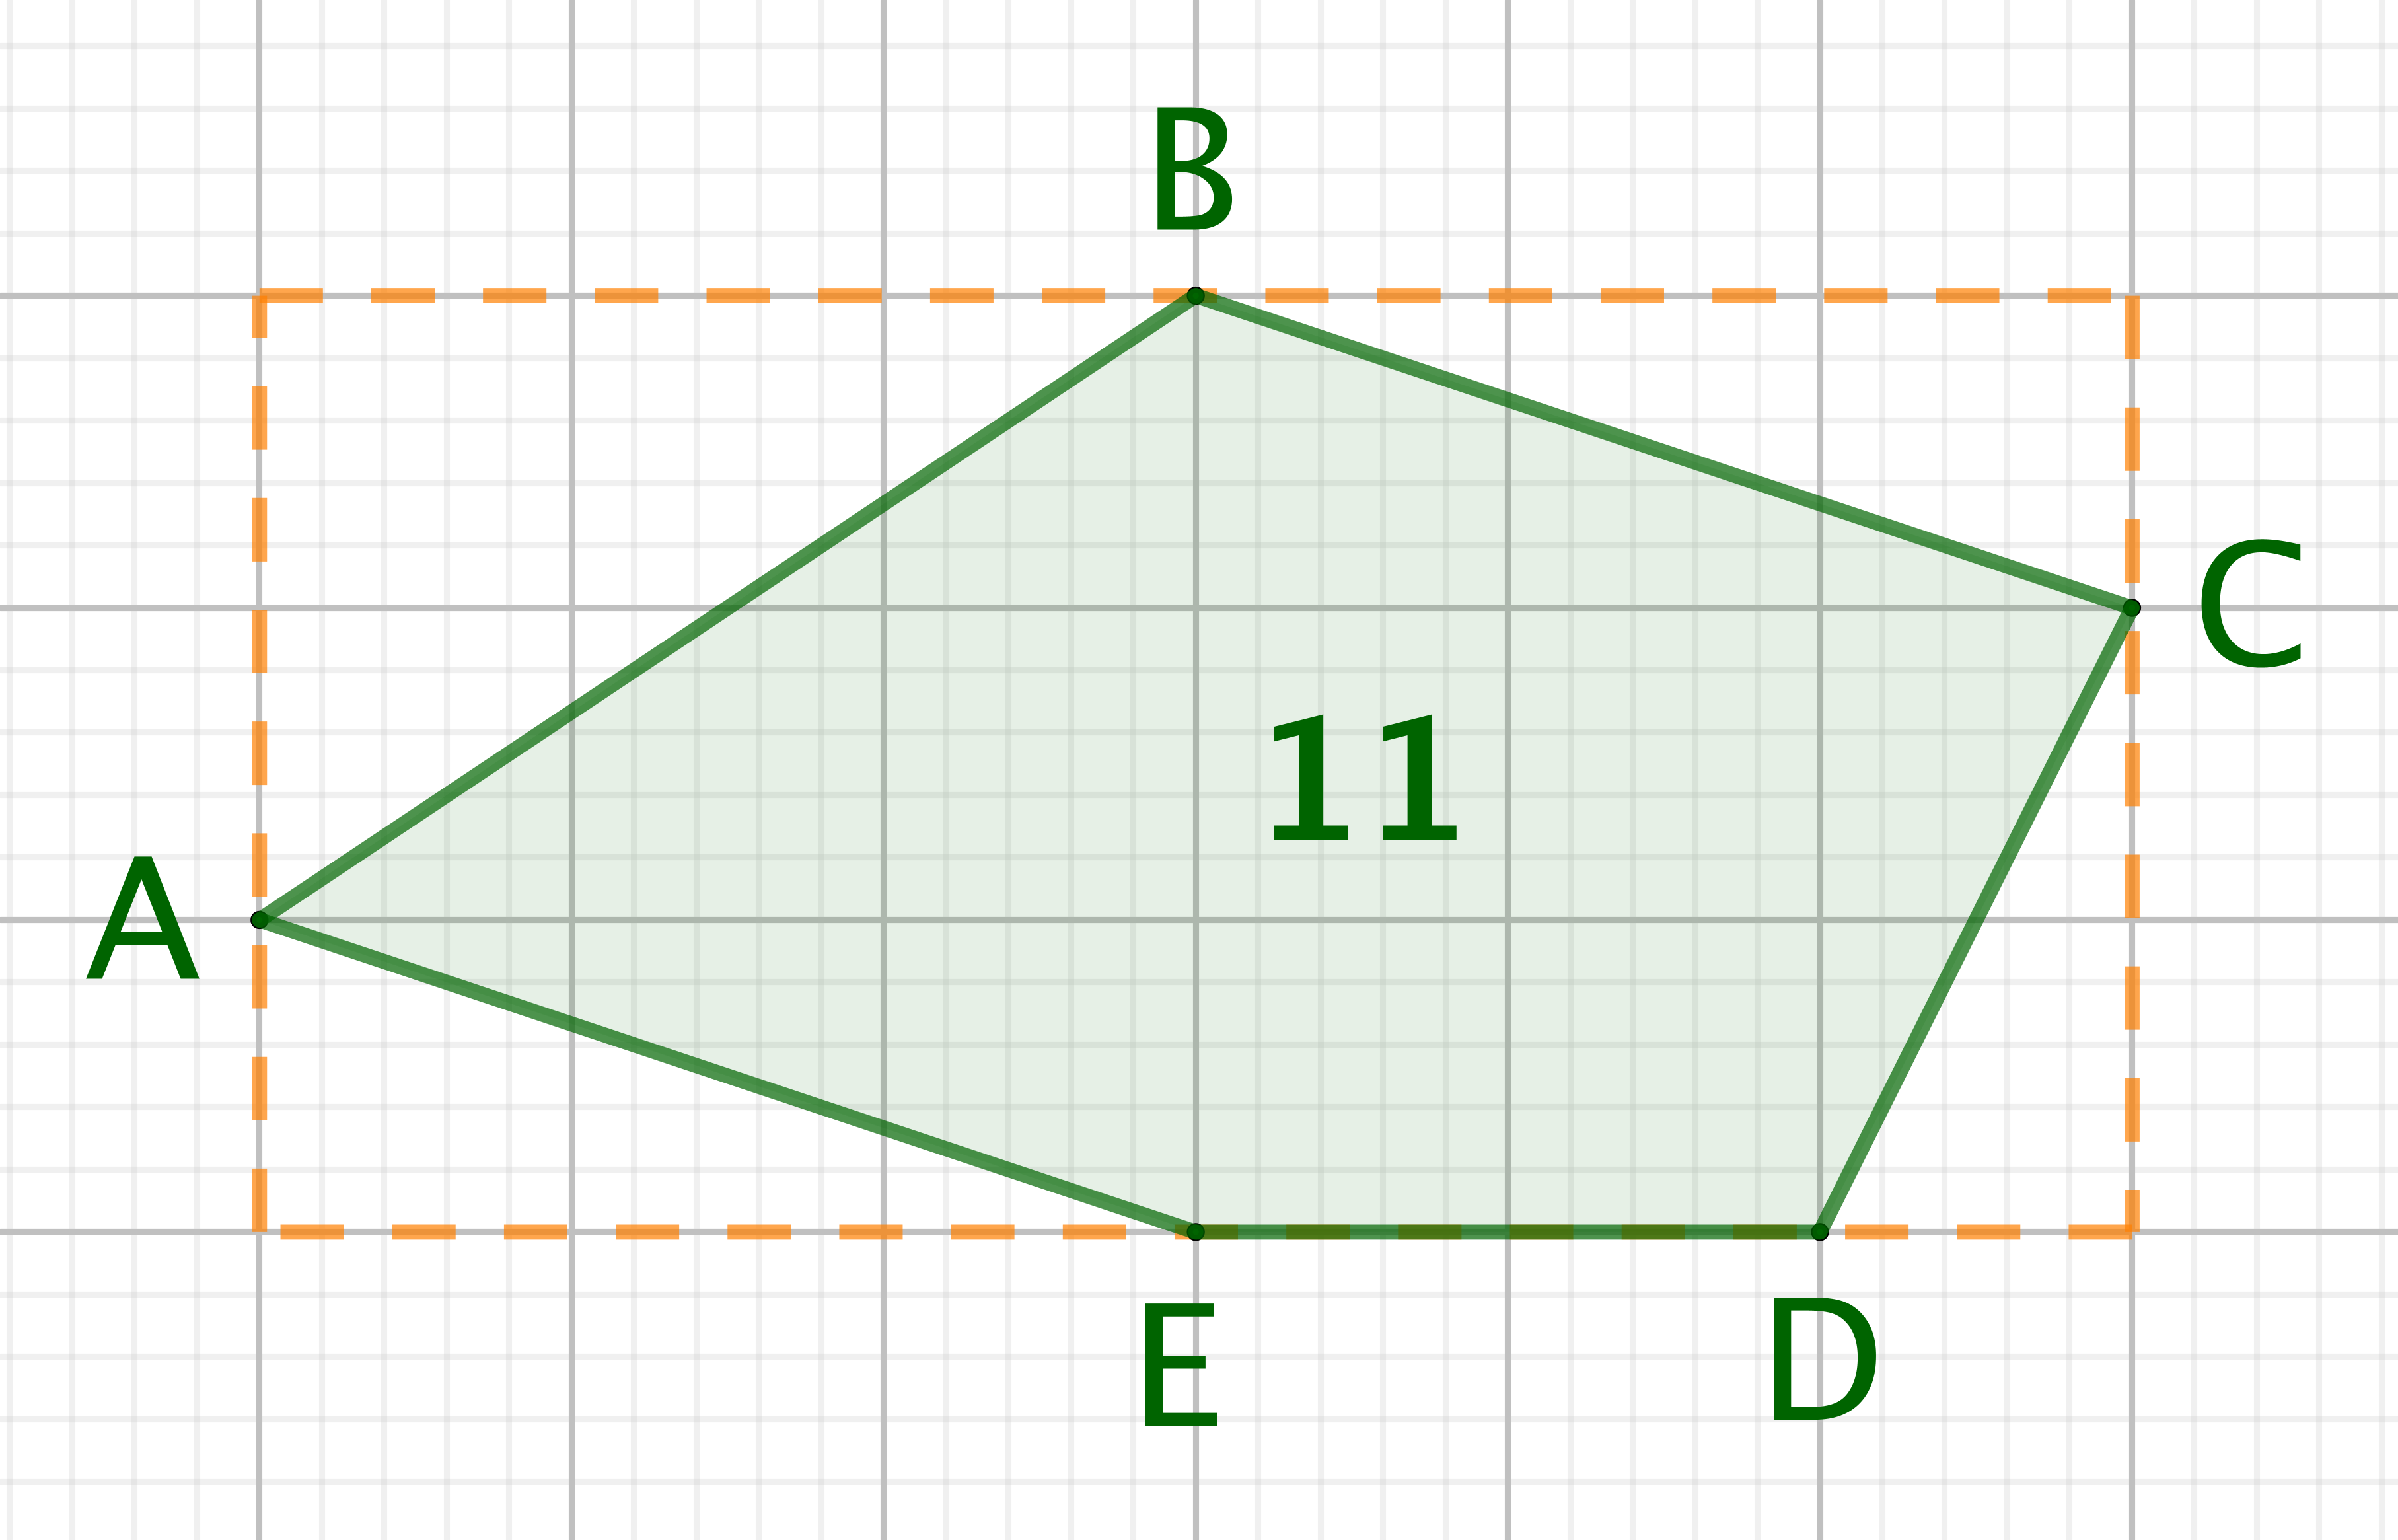
\includegraphics[scale=.35]{content/polygon/at-least-one/convex-1.png}
%
%       	\smallskip
%
%		$11 = 3 \cdot 6 - \dfrac{3 \cdot 1 + 3 \cdot 2 + 3 \cdot 1 + 1 \cdot 2}{2} \vphantom{\dfrac{2^M}2}$
%    \end{center}
%
%	\columnbreak
%
%    \begin{center}
%		Via le déterminant.
%
%		\smallskip
%
%        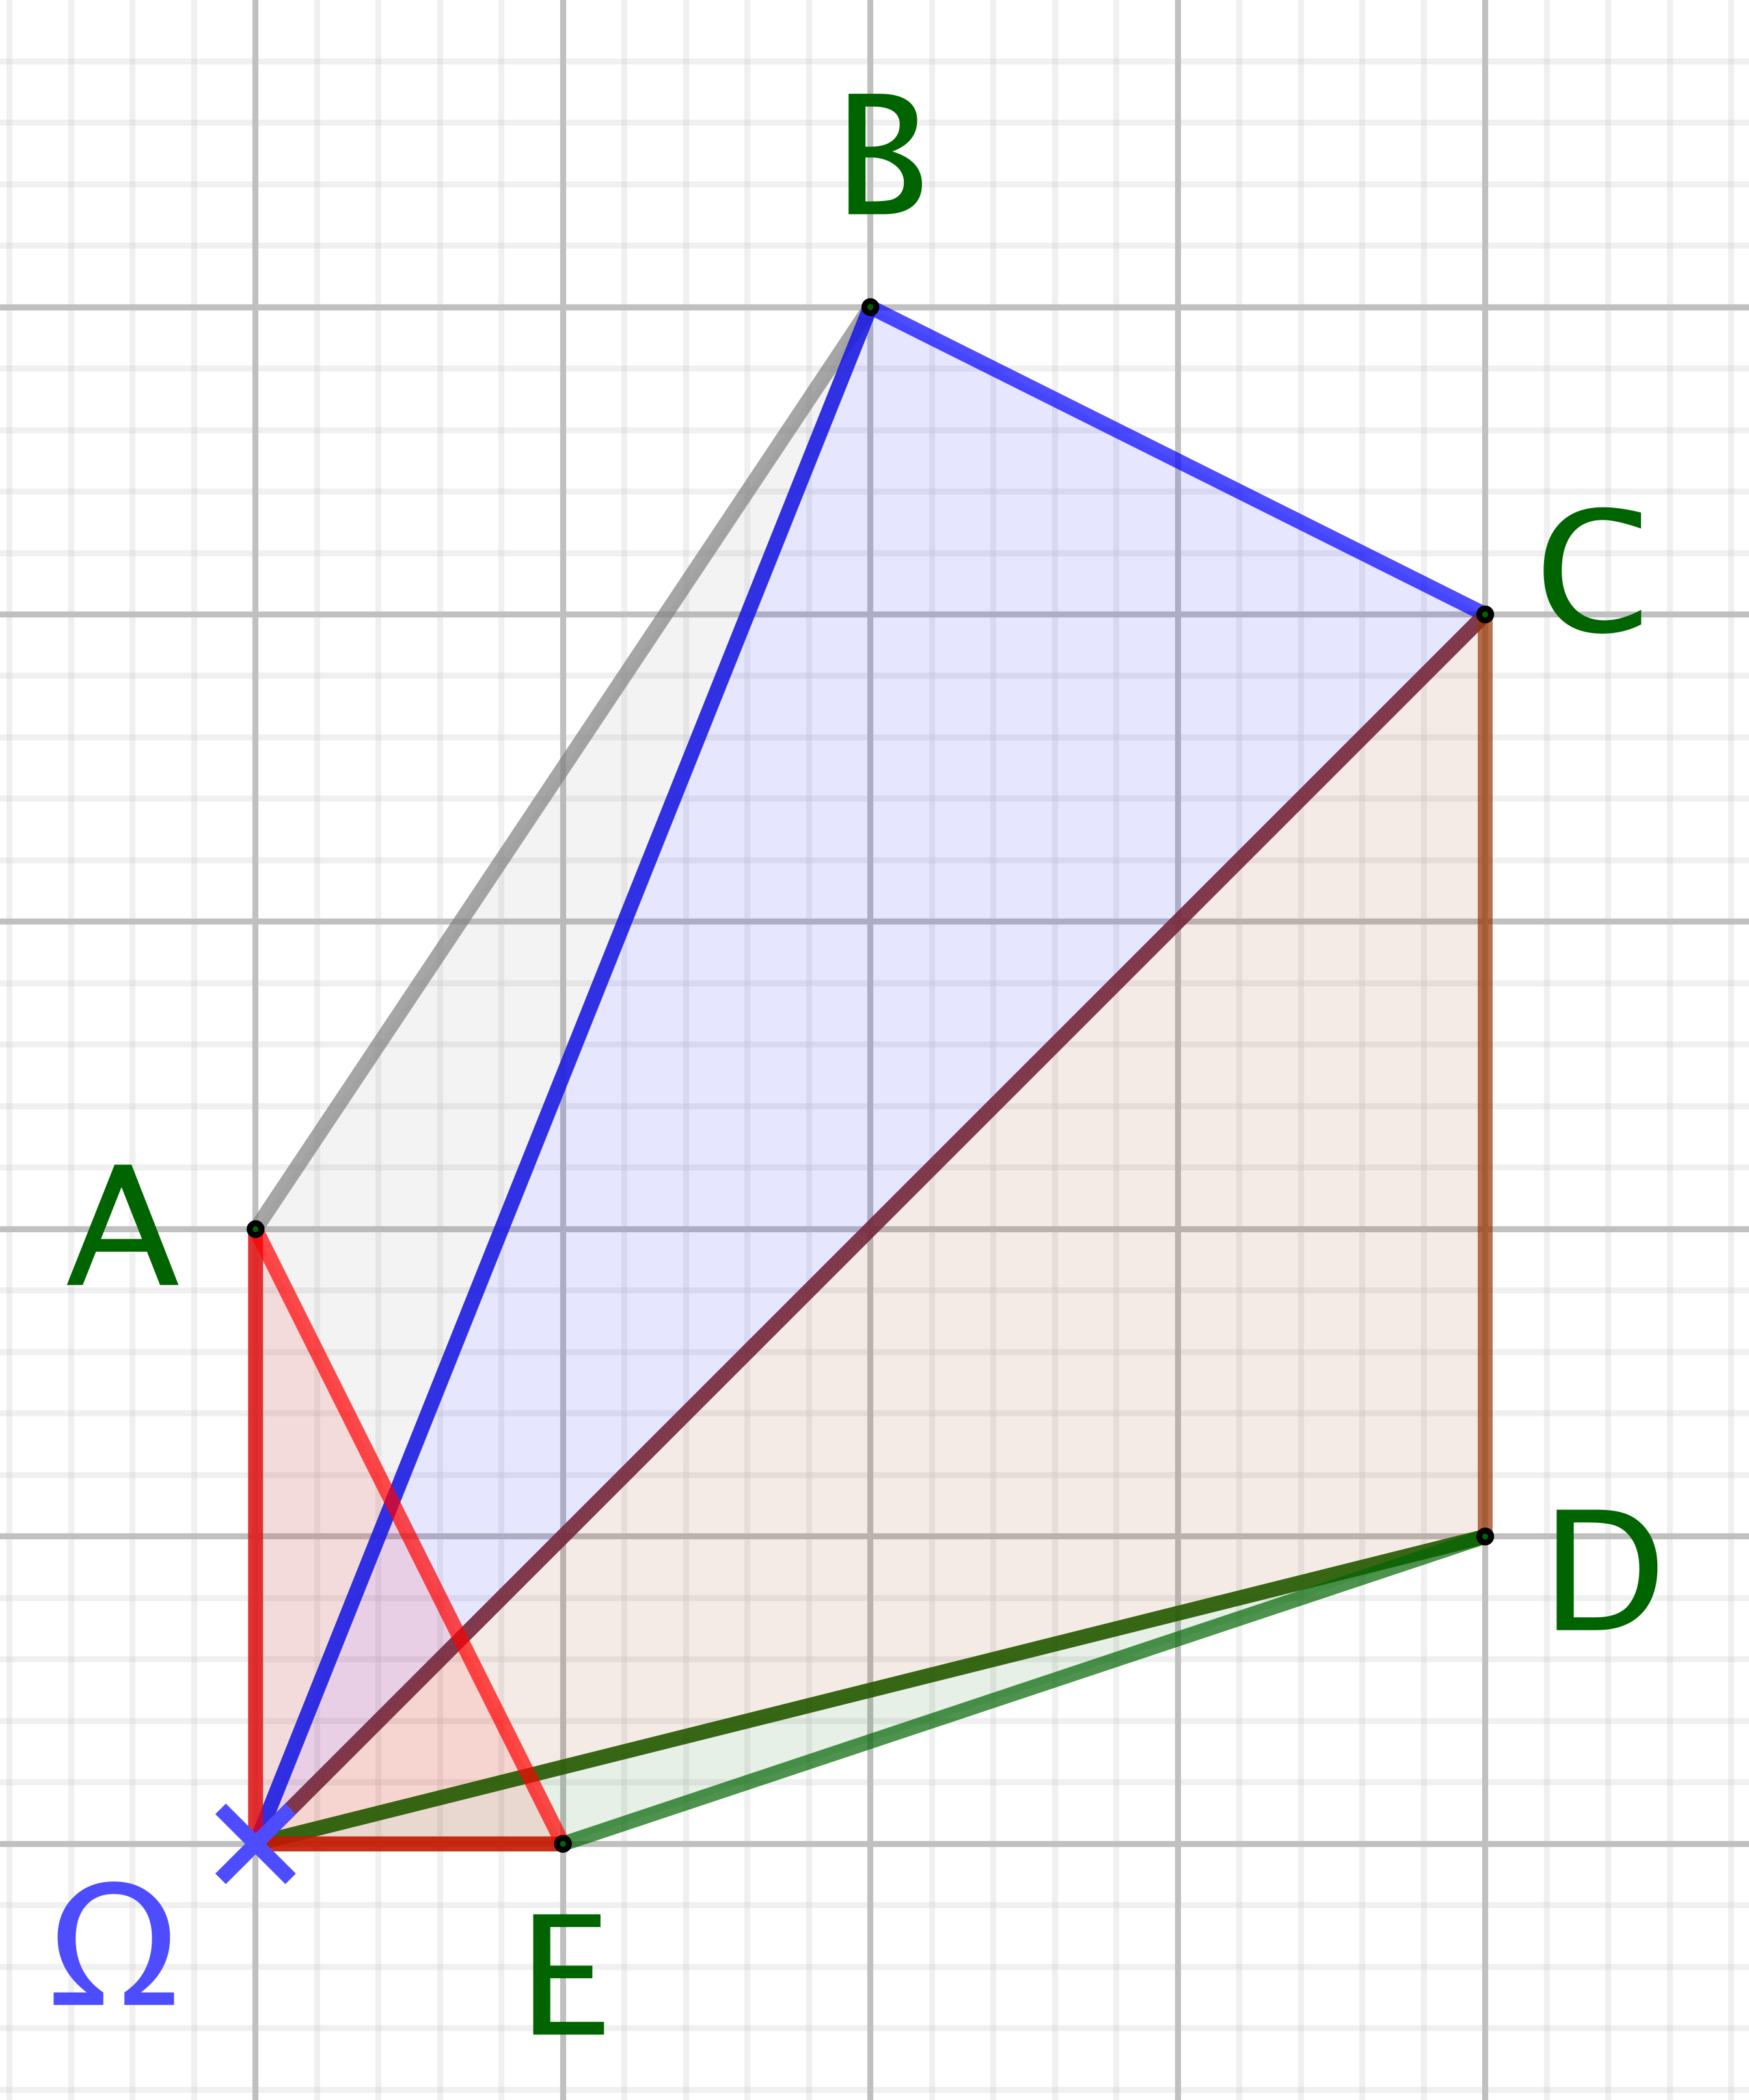
\includegraphics[scale=.35]{content/polygon/at-least-one/convex-2.png}
%
%       	\smallskip
%
%		$- 11 = 3 - \num{1.5} - \num{6.5} - 3 - 3 \vphantom{\dfrac{2^M}2}$
%    \end{center}
%\end{multicols}
%
%
%Dans le cas précédent, le résultat pourrait dépendre du point $\Omega$ employé, mais le fait suivant nous montre que non. Allons-y!
%
%
%% ----------------------- %
%
%
%\begin{fact} \label{garea-pt-ct}
%    Soit $\setproba{L} = A_1 A_2 \cdots A_n$ un \ncycle.
%    La fonction qui à un point $\Omega$ du plan associe
%    $\mu_1^n (\Omega ;\setproba{L}) = \dsum_{i=1}^{n} \det \big( \vect{\Omega A^{\,\prime}_i} , \vect{\Omega A^{\,\prime}_{i+1}} \big)$ est indépendante du point $\Omega$.
%    Dans la suite, cette quantité indépendante de $\Omega$ sera notée $\mu_1^n (\setproba{L})$.
%\end{fact}
%
%
%\begin{proof}
%    Soit $M$ un autre point du plan.
%
%    \begin{stepcalc}[style=ar*]
%        \mu_1^n (\Omega ;\setproba{L})
%    \explnext{}
%        \dsum_{i=1}^{n} \det \big( \vect{\Omega A^{\,\prime}_i} , \vect{\Omega A^{\,\prime}_{i+1}} \big)
%    \explnext*{Cette bonne vieille relation de Chasles.}{}
%        \dsum_{i=1}^{n} \det \big( \vect{\Omega M} + \vect{M A^{\,\prime}_i} , \vect{\Omega M} + \vect{M A^{\,\prime}_{i+1}} \big)
%    \explnext{}
%        \dsum_{i=1}^{n} \Big[
%            \det \big( \vect{\Omega M} , \vect{\Omega M} \big)
%            +
%            \det \big( \vect{\Omega M} , \vect{M A^{\,\prime}_{i+1}} \big)
%            +
%            \det \big( \vect{M A^{\,\prime}_i} , \vect{\Omega M} \big)
%            +
%            \det \big( \vect{M A^{\,\prime}_i} , \vect{M A^{\,\prime}_{i+1}} \big)
%        \Big]
%    \explnext{}
%        \dsum_{i=1}^{n} \det \big( \vect{\Omega M} , \vect{M A^{\,\prime}_{i+1}} \big)
%        +
%        \dsum_{i=1}^{n} \det \big( \vect{M A^{\,\prime}_i} , \vect{\Omega M} \big)
%        +
%        \mu_1^n (M ; \setproba{L})
%    \explnext{}
%        \mu_1^n (M ; \setproba{L})
%        +
%        \dsum_{i=2}^{n+1} \det \big( \vect{\Omega M} , \vect{M A^{\,\prime}_{i}} \big)
%        -
%        \dsum_{i=1}^{n} \det \big( \vect{\Omega M} , \vect{M A^{\,\prime}_i} \big)
%    \explnext*{$A^{\,\prime}_{n+1} = A^{\,\prime}_1$}{}
%        \mu_1^n (M ; \setproba{L})
%    \end{stepcalc}
%
%    \null\vspace{-3.5ex}
%\end{proof}
%
%
%% ----------------------- %
%
%
%\begin{fact} \label{nline-shift-inva}
%    Soit $\setproba{L} = A_1 A_2 \cdots A_n$ un \ncycle.
%    Pour $k \in \ZintervalC{1}{n}$,
%    le \ncycle\ $\setproba{L}_j = B_1 B_2 \cdots B_n$, où $B_i = A^{\,\prime}_{i+k-1}$,
%    vérifie
%    $\mu_1^n (\setproba{L}) = \mu_1^n (\setproba{L}_k)$.
%    Dans la suite, cette quantité commune sera notée $\mu (\setproba{L})$.
%\end{fact}
%
%
%\begin{proof}
%    Il suffit de s'adonner à un petit jeu sur les indices de sommation.
%\end{proof}
%
%
%% ----------------------- %
%
%
%\begin{fact} \label{nline-rota-inva}
%    Soit
%    $\setproba{L} = A_1 A_2 \cdots A_n$ un \ncycle.
%    Le \ncycle\ $\setproba{L}^{\mathrm{op}} = B_1 B_2 \cdots B_n$, où $B_i =  A_{n + 1 - i}$,
%    vérifie
%    $\mu(\setproba{L}^{\mathrm{op}}) = {} - \mu(\setproba{L})$.
%\end{fact}
%
%
%\begin{proof}
%    Soit $\Omega$ un point quelconque du plan.
%
%    \begin{stepcalc}[style=ar*]
%        \mu(\setproba{L}^{\mathrm{op}})
%    \explnext{}
%        \dsum_{i=1}^{n} \det \big( \vect{\Omega B^{\,\prime}_i} , \vect{\Omega B^{\,\prime}_{i+1}} \big)
%    \explnext{}
%        \dsum_{i=1}^{n} \det \big( \vect{\Omega A^{\,\prime}_{n + 1 - i}} , \vect{\Omega A^{\,\prime}_{n - i}} \big)
%    \explnext{}
%        \dsum_{j=0}^{n-1} \det \big( \vect{\Omega A^{\,\prime}_{j + 1}} , \vect{\Omega A^{\,\prime}_j} \big)
%    \explnext*{$A^{\,\prime}_0 = A^{\,\prime}_n$ et $A^{\,\prime}_1 = A^{\,\prime}_{n+1}$}{}
%        \dsum_{j=1}^{n} \det \big( \vect{\Omega A^{\,\prime}_{j + 1}} , \vect{\Omega A^{\,\prime}_j} \big)
%    \explnext{}
%        {} - \dsum_{j=1}^{n} \det \big( \vect{\Omega A^{\,\prime}_j} , \vect{\Omega A^{\,\prime}_{j + 1}} \big)
%    \explnext{}
%        {} - \mu(\setproba{L})
%    \end{stepcalc}
%
%    \null\vspace{-3.5ex}
%\end{proof}
%
%
%% ----------------------- %
%
%
%\begin{fact} \label{garea-ncycle}
%    Soit
%    $\setproba{L} = A_1 A_2 \cdots A_n$ un \ncycle.
%    La quantité $\frac12 \mu(\setproba{L})$, qui dépend juste du sens de parcours de $\setproba{L}$, mais pas du point de départ choisi,%
%    \footnote{
%        Le lecteur pardonnera les abus de langage utilisés.
%    }
%    sera appelé \og \emph{aire algébrique} \fg\ de $\setproba{L}$.
%\end{fact}
%
%
%\begin{proof}
%    C'est une conséquence directe des faits \ref{nline-shift-inva} et \ref{nline-rota-inva}.
%\end{proof}
%
%% ----------------------- %
%
%
%Considérons, maintenant, un \ngone\ convexe $\setproba{P} = A_1 A_2 \cdots A_n$. En choisissant l'isobarycentre $G$ des sommets $A_1$, $A_2$, ..., $A_n$ pour le calcul de $\mu(\setproba{P})$, nous obtenons que $\area{\setproba{P}} = \frac12  \abs{\mu(\setproba{P})}$:
%en effet,
%avec ce choix, tous les déterminants $\det \big( \vect{G A^{\,\prime}_i} , \vect{G A^{\,\prime}_{i+1}} \big)$ ont le même signe.
%Dans le cas non-convexe, les choses se compliquent a priori, car nous ne maîtrisons plus les signes des déterminants. Heureusement, nous avons le résultat suivant.
%
%
%\begin{fact} \label{route-direction}
%    Soit un \ngone\ $\setproba{P} = A_1 A_2 \cdots A_n$ tel que $A_1$, $A_2$, ..., $A_n$ soient parcourus dans le sens trigonométrique, ou anti-horaire.
%    Un tel \ngone\ sera dit \og \emph{positif} \fg.%
%    \footnote{
%    	Bien noté que cette notion ne peut pas exister pour un \ngone\ croisé. De façon cachée, nous utilisons le célèbre théorème de Jordan, dans sa forme polygonale.
%    }
%    Sous cette hypothèse, nous avons $\mu(\setproba{P}) \geq 0$.
%\end{fact}
%
%
%\begin{proof}
%	Le théorème de triangulation affirme que tout \ngone\ est triangulable comme dans l'exemple très basique suivant qui laisse envisager une démonstration par récurrence en retirant l'un des triangles ayant deux côtés correspondant à deux côtés consécutifs du \ngone\ (pour peu qu'un tel triangle existe toujours).
%
%
%    \begin{multicols}{3}
%        \small\itshape
%        \begin{center}
%            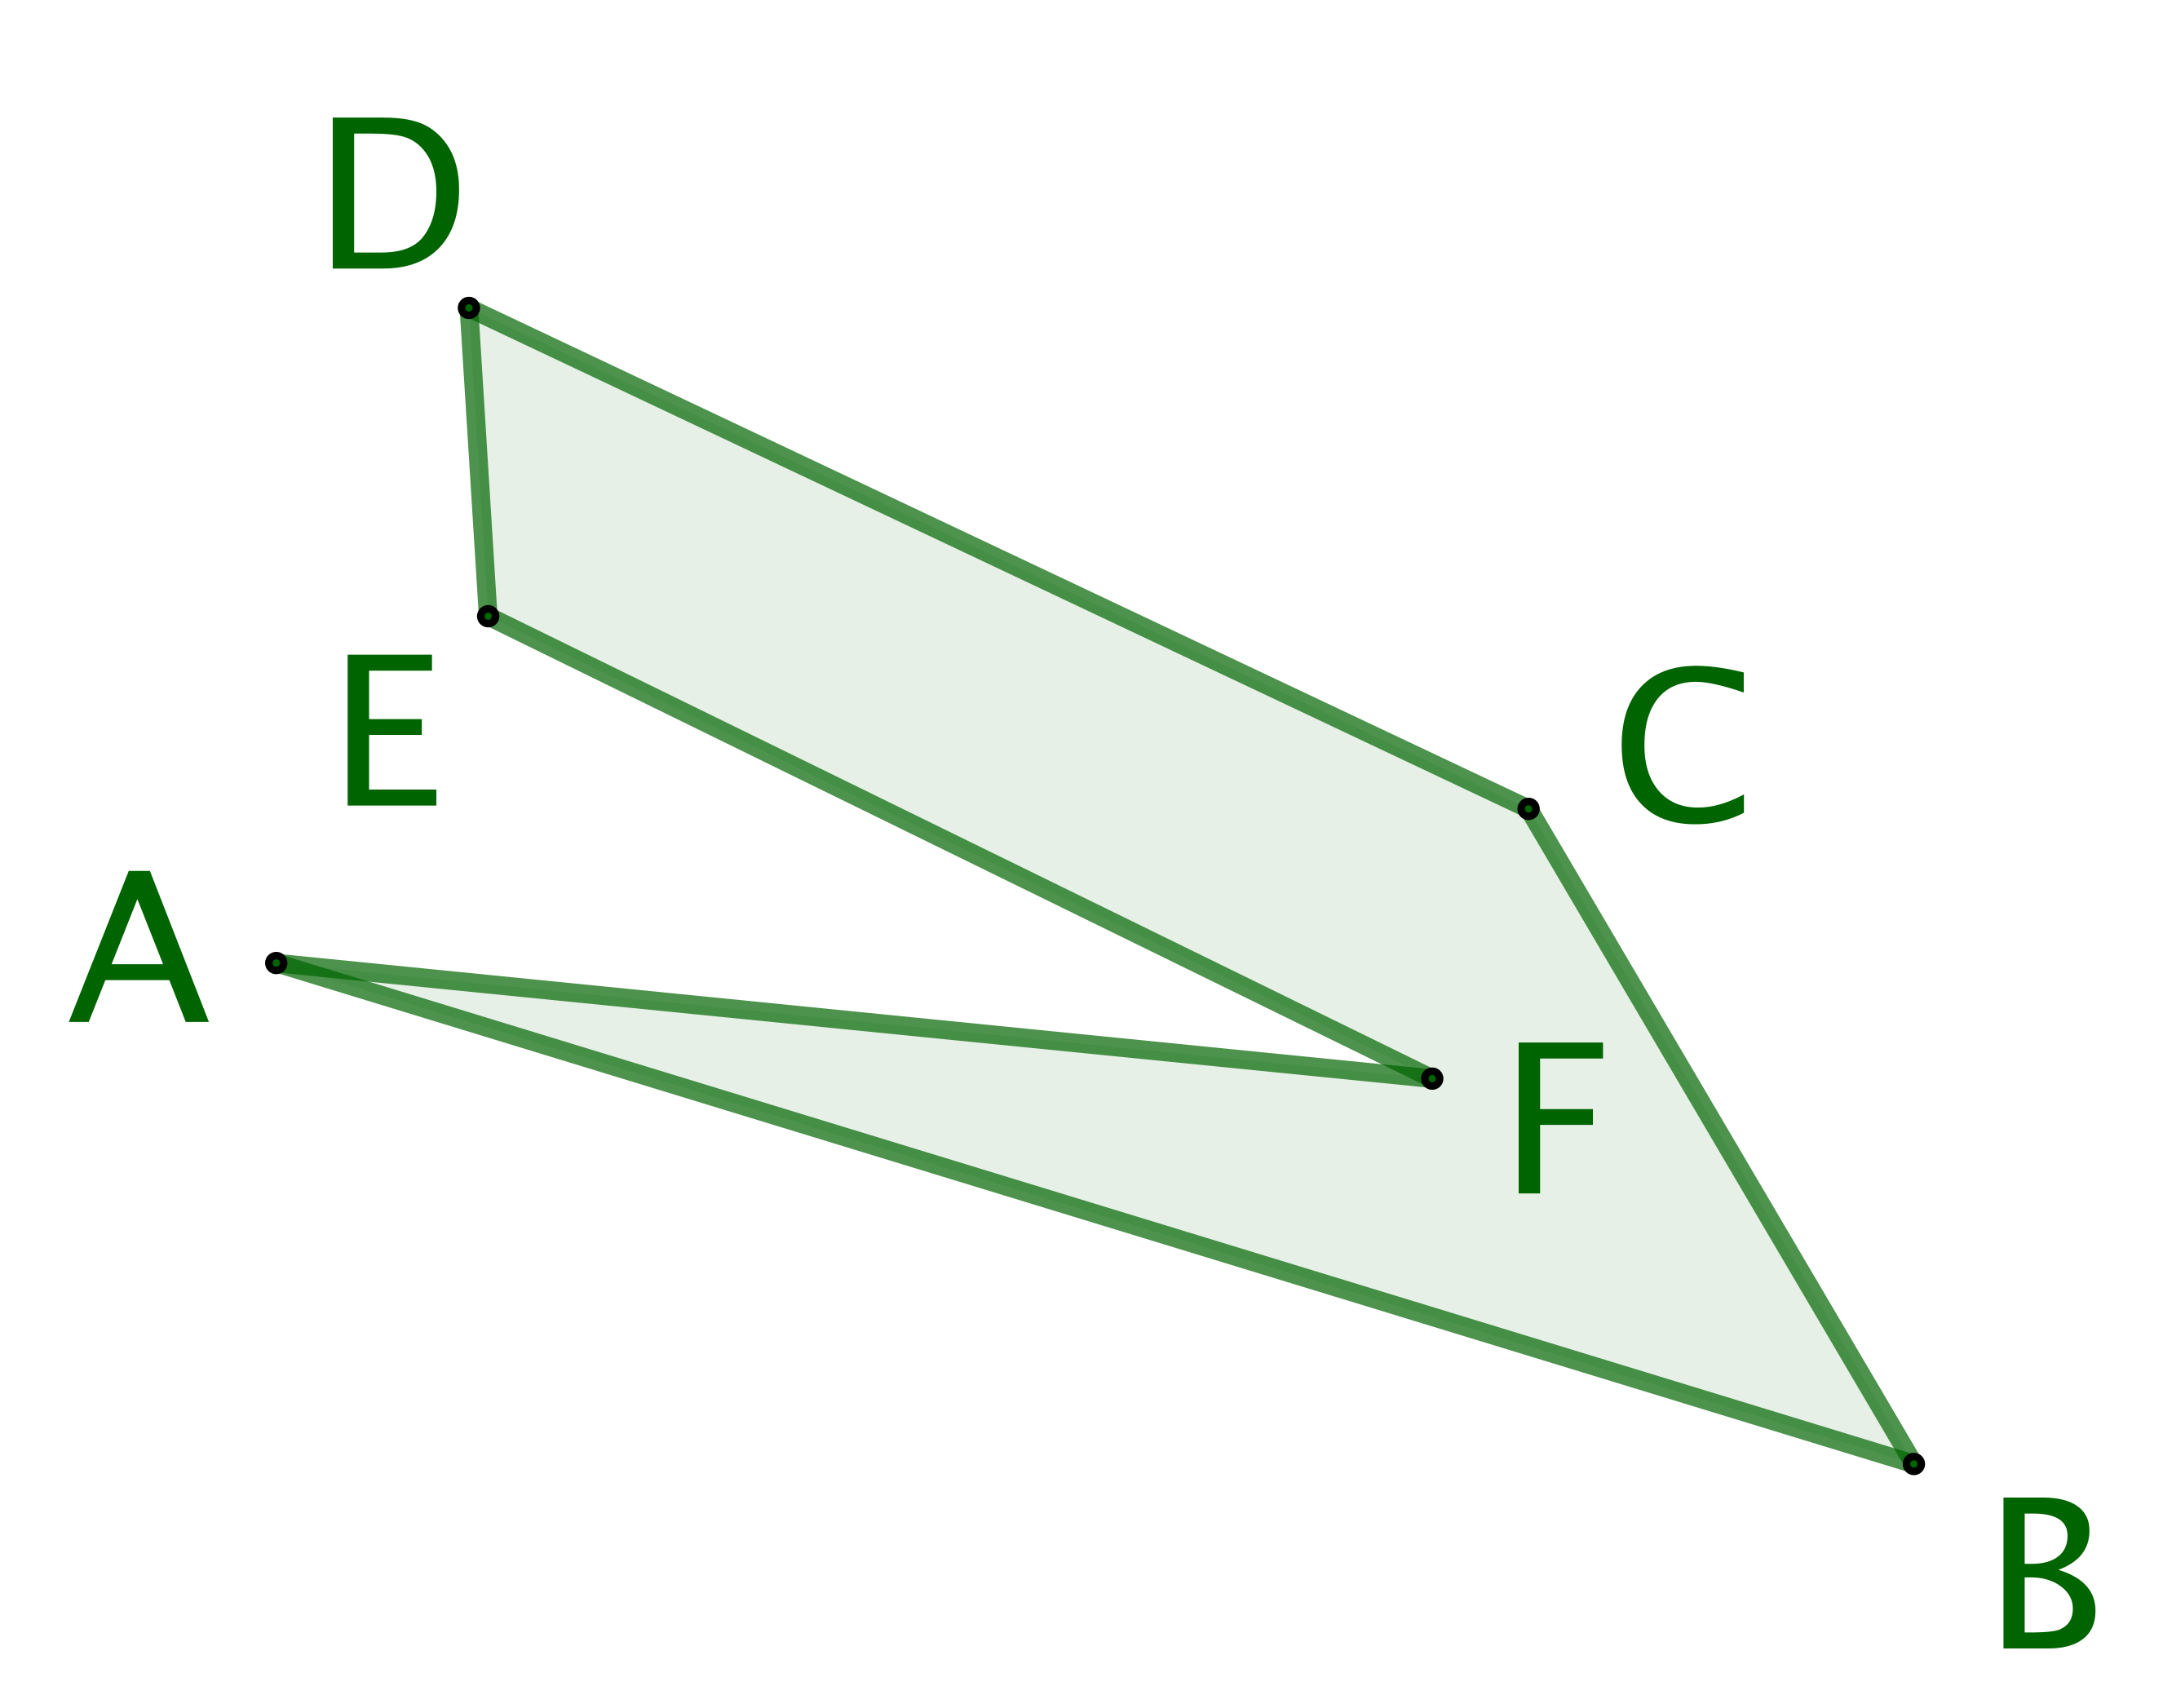
\includegraphics[scale=.4]{content/polygon/at-least-one/triangulation-1.png}
%
%            \smallskip
%            Un \ngone\ \og nu \fg.
%        \end{center}
%
%
%        \begin{center}
%            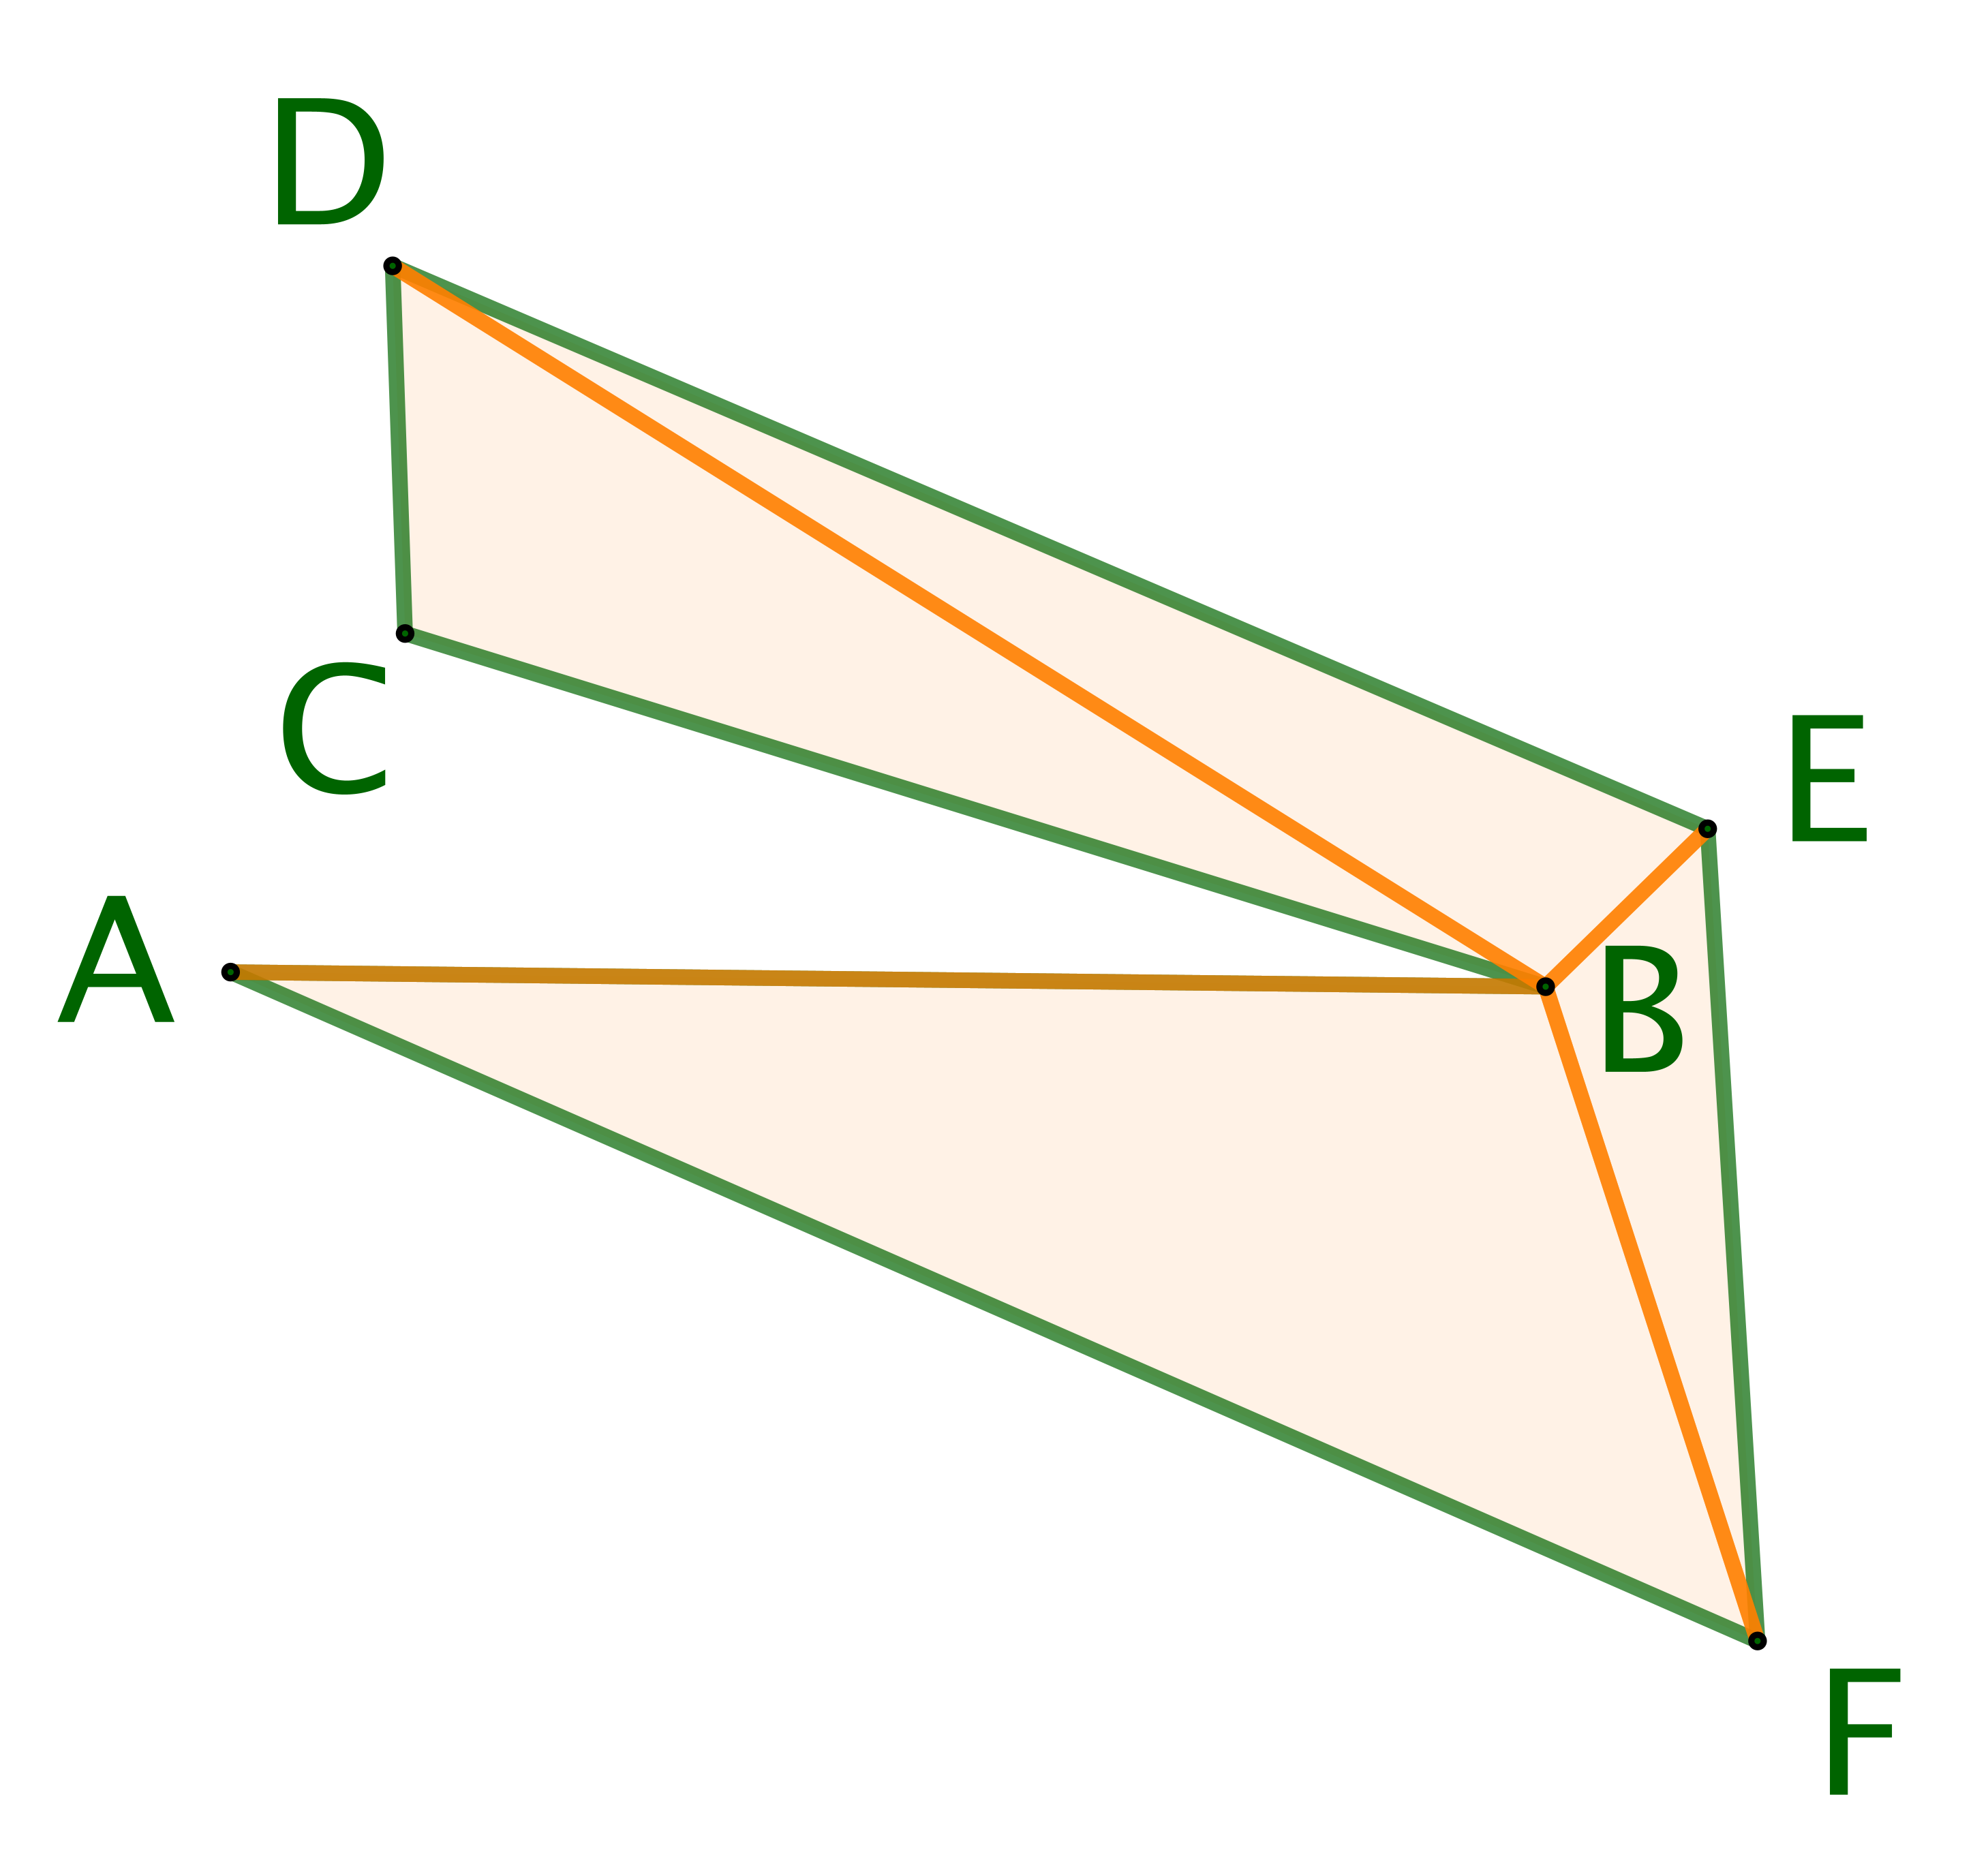
\includegraphics[scale=.4]{content/polygon/at-least-one/triangulation-2.png}
%
%            \smallskip
%            Le \ngone\ triangulé.
%        \end{center}
%
%
%        \begin{center}
%            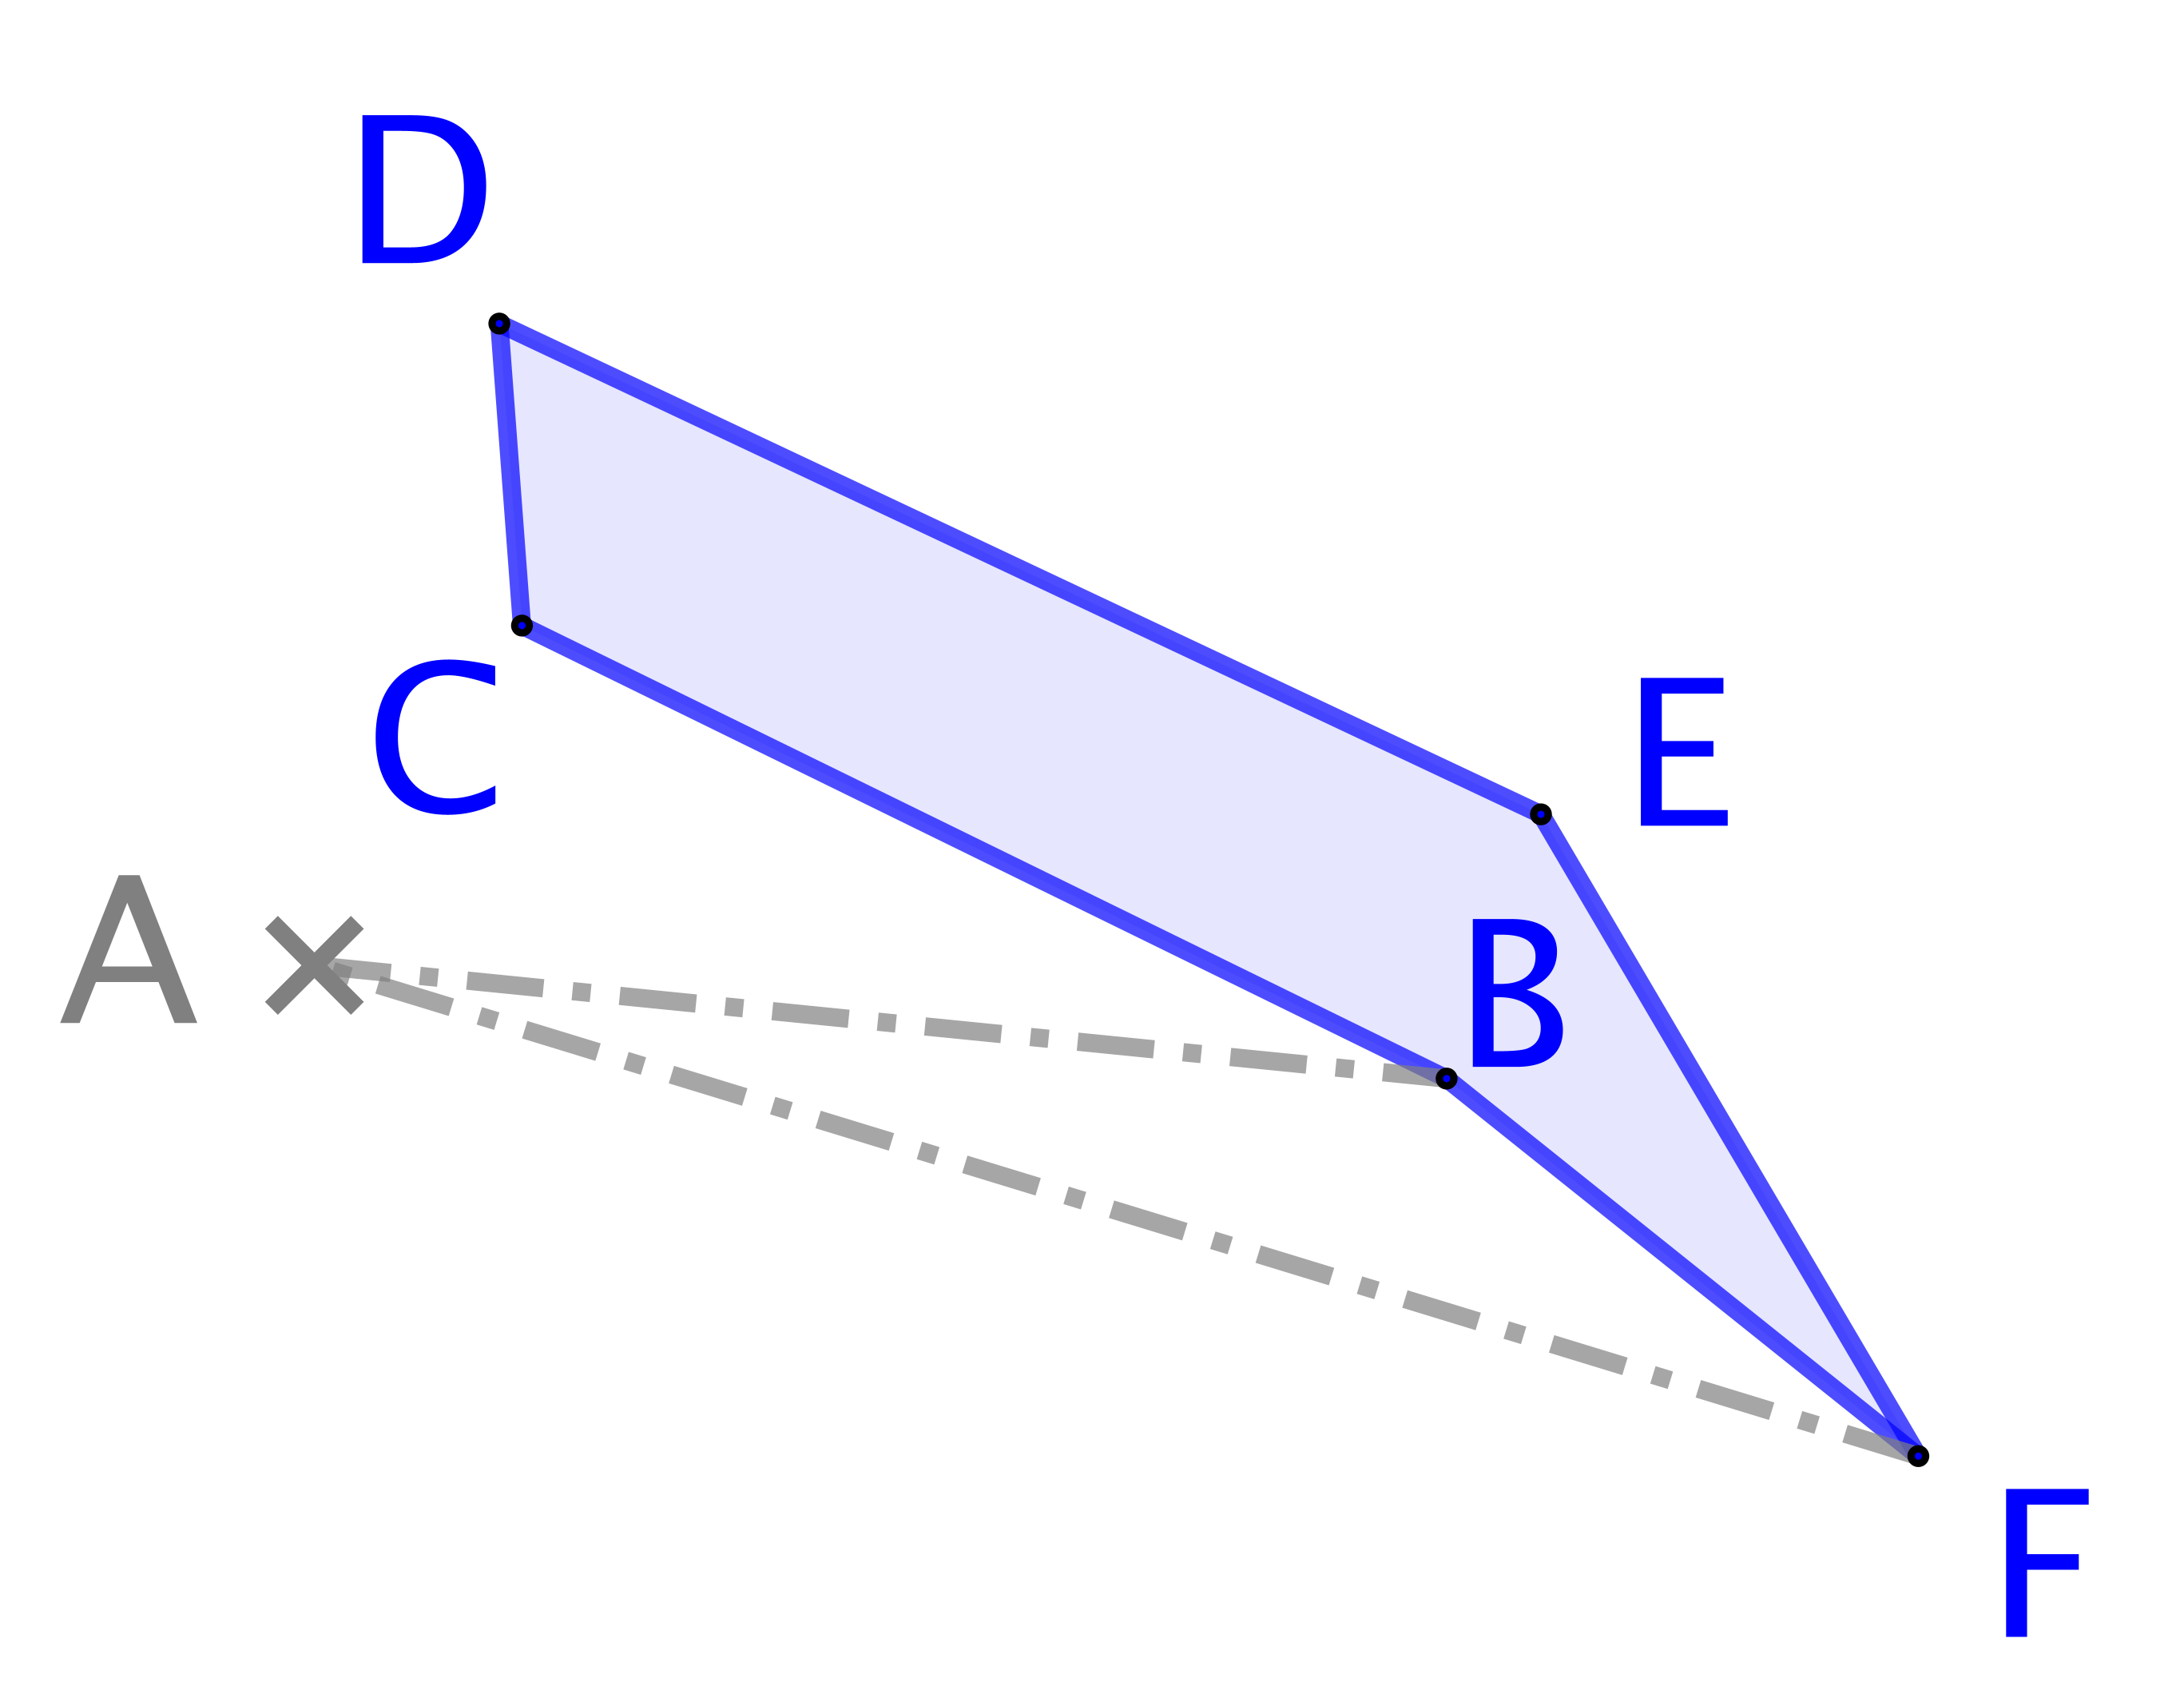
\includegraphics[scale=.4]{content/polygon/at-least-one/triangulation-3.png}
%
%            \smallskip
%            Le \ngone\ allégé.
%        \end{center}
%    \end{multicols}
%
%
%    Le théorème de triangulation admet une forme forte donnant une décomposition contenant un triangle formé de deux côtés consécutifs du \ngone.%
%    \footnote{
%        En pratique, cette forme forte est peu utile, car elle aboutit à un algorithme de recherche trop lent.
%    }
%    Nous dirons qu'une telle décomposition est \og \emph{à l'écoute} \fg.
%    Ce très mauvais jeu de mots fait référence à la notion sérieuse \og \emph{d'oreille} \fg\ pour un \ngone: une oreille est un triangle inclus dans le \ngone, et formé de deux côtés consécutifs du \ngone.
%    L'exemple suivant donne un \ngone\ n'ayant que deux oreilles.%
%    \footnote{
%        On démontre que tout \ngone\ admet au minimum deux oreilles.
%    }
%
%
%    \begin{multicols}{2}
%        \small\itshape
%    	\begin{center}
%        	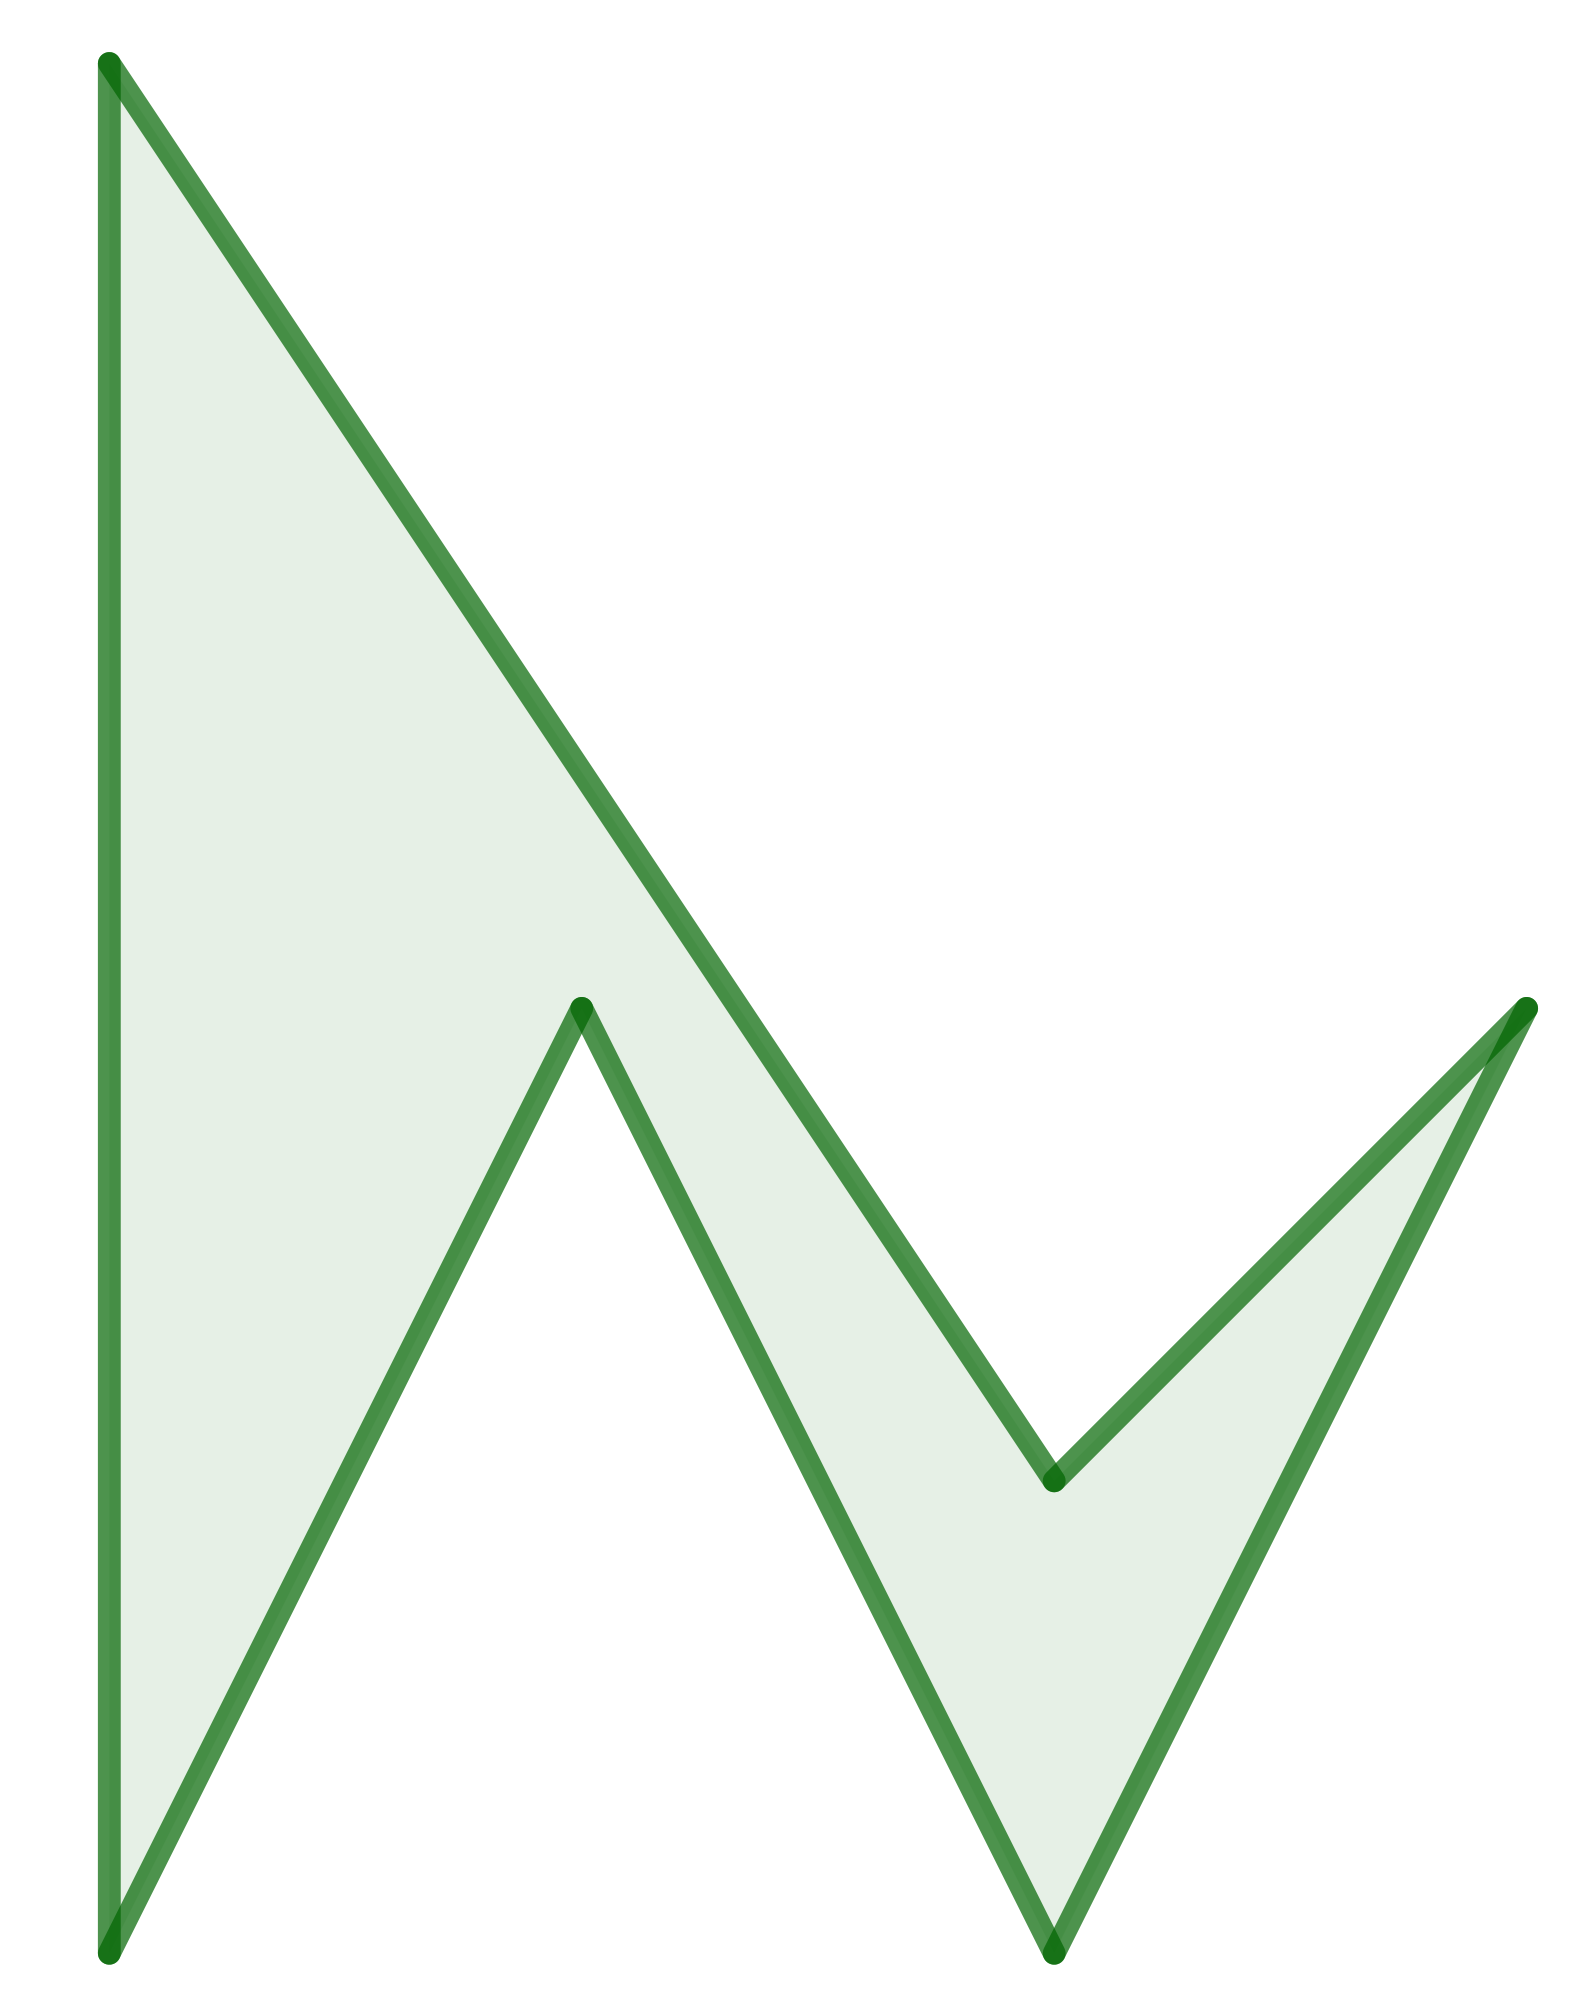
\includegraphics[scale=.4]{content/polygon/at-least-one/mini-ear-1.png}
%
%        	\smallskip
%       		Un \ngone\ basique.
%    	\end{center}
%
%    	\begin{center}
%        	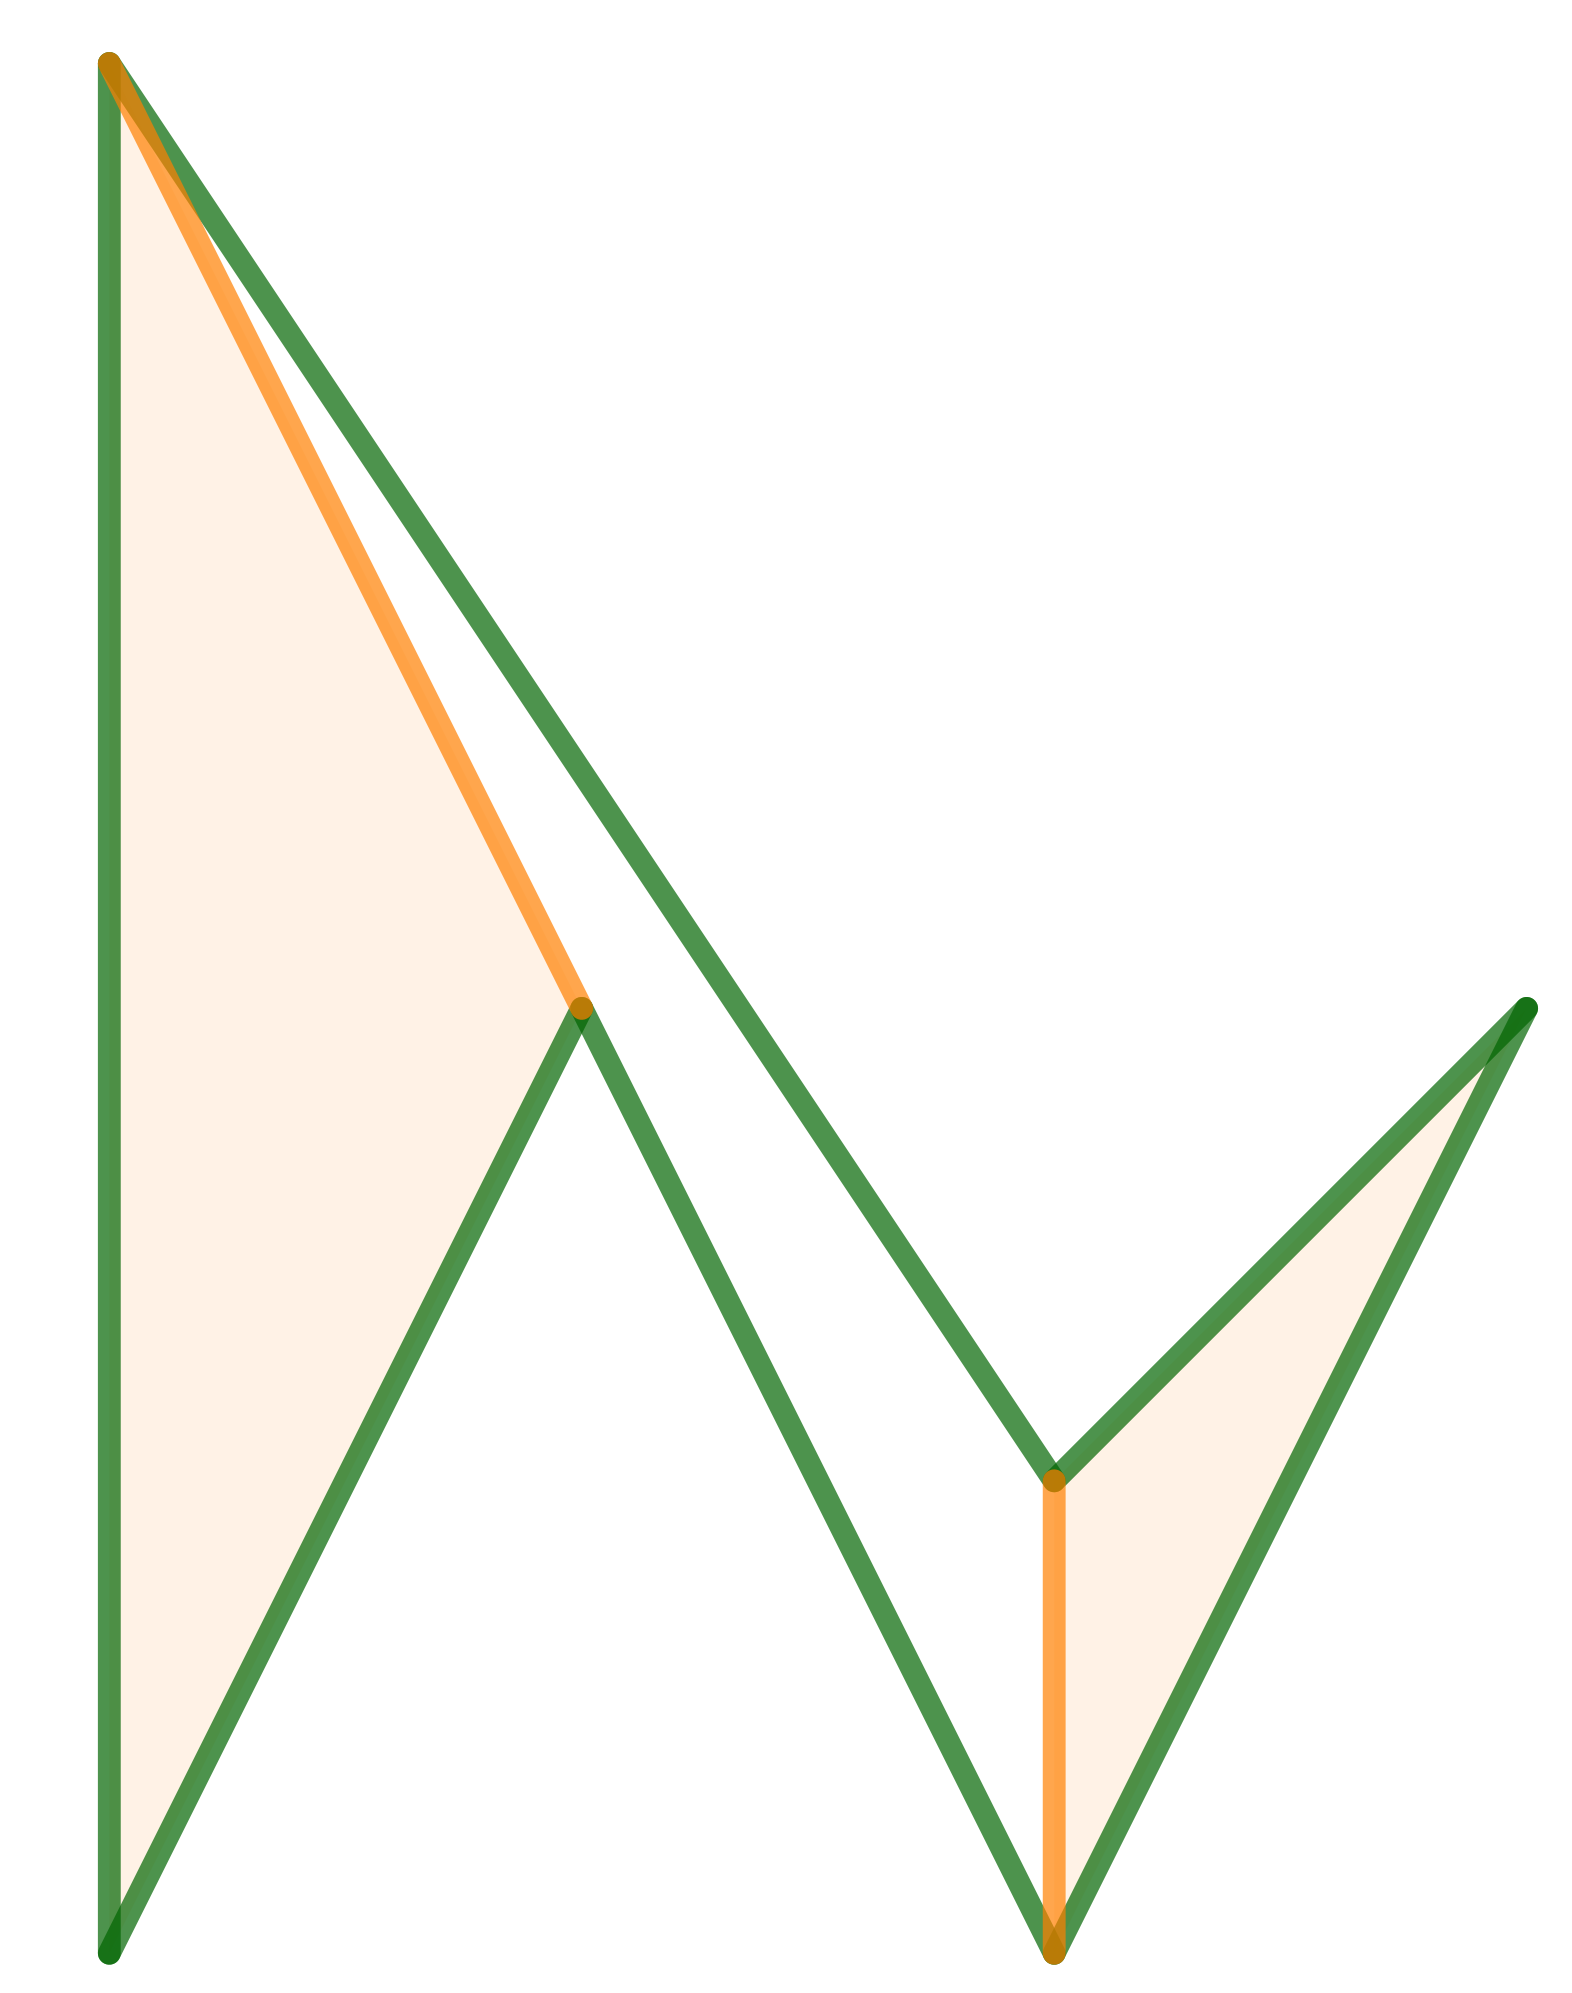
\includegraphics[scale=.4]{content/polygon/at-least-one/mini-ear-2.png}
%
%        	\smallskip
%       		Juste deux oreilles disponibles.
%    	\end{center}
%    \end{multicols}
%
%
%	Raisonnons donc par récurrence sur $n \in \NN_{\geq3}$.
%
%	\begin{itemize}
%		\item \textbf{Cas de base.}
%		Soit $ABC$ un triangle. Dire que les sommets $A$, $B$ et $C$ sont parcourus dans le sens trigonométrique, c'est savoir que $\mu(ABC) = \det \big( \vect{AB} , \vect{AC} \big) > 0$.
%
%
%		\item \textbf{Hérédité.}
%		Soit un \ngone\ positif $\setproba{P} = A_1 A_2 \cdots A_n$ avec $n \in \NN_{>3}$. On peut supposer que $A_{n-1} A_n A_1$ est une oreille d'une triangulation à l'écoute du \ngone\ $\setproba{P}$.
%
%
%	    \begin{multicols}{2}
%    	    \small\itshape
%    		\begin{center}
%        	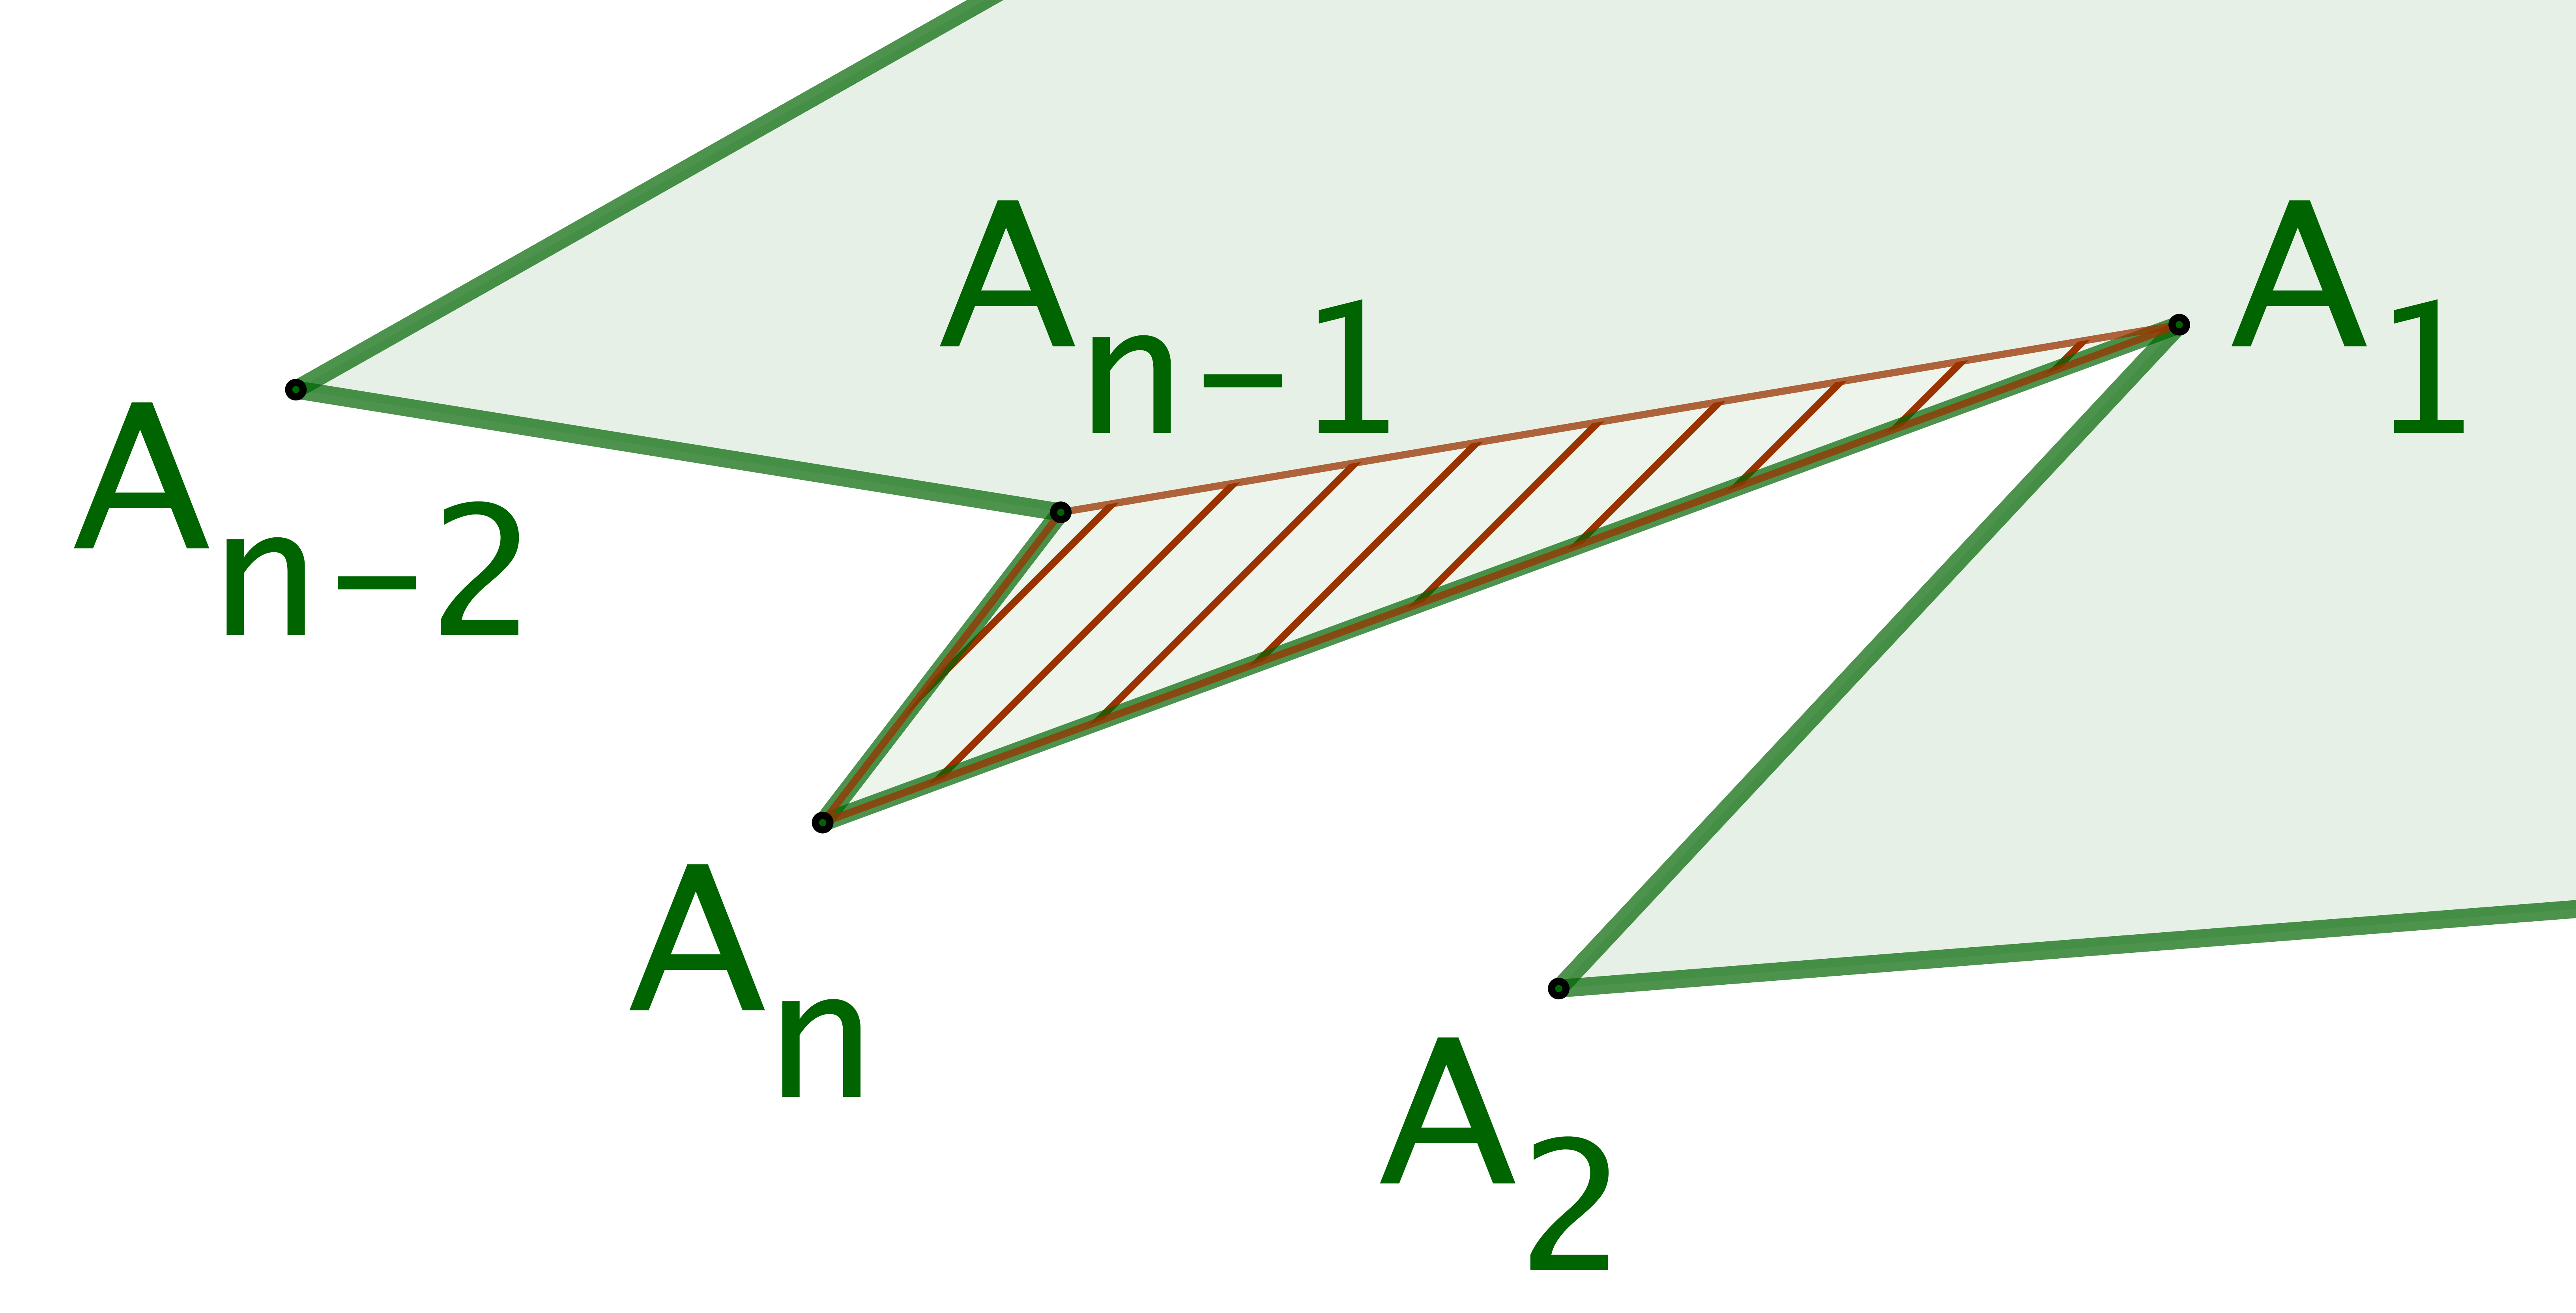
\includegraphics[scale=.4]{content/polygon/at-least-one/triangulation-proof-OK.png}
%
%	        	\smallskip
%    	   		$A_{n-1} A_n A_1$ est une oreille.
%    	\end{center}
%
%	    	\begin{center}
%        	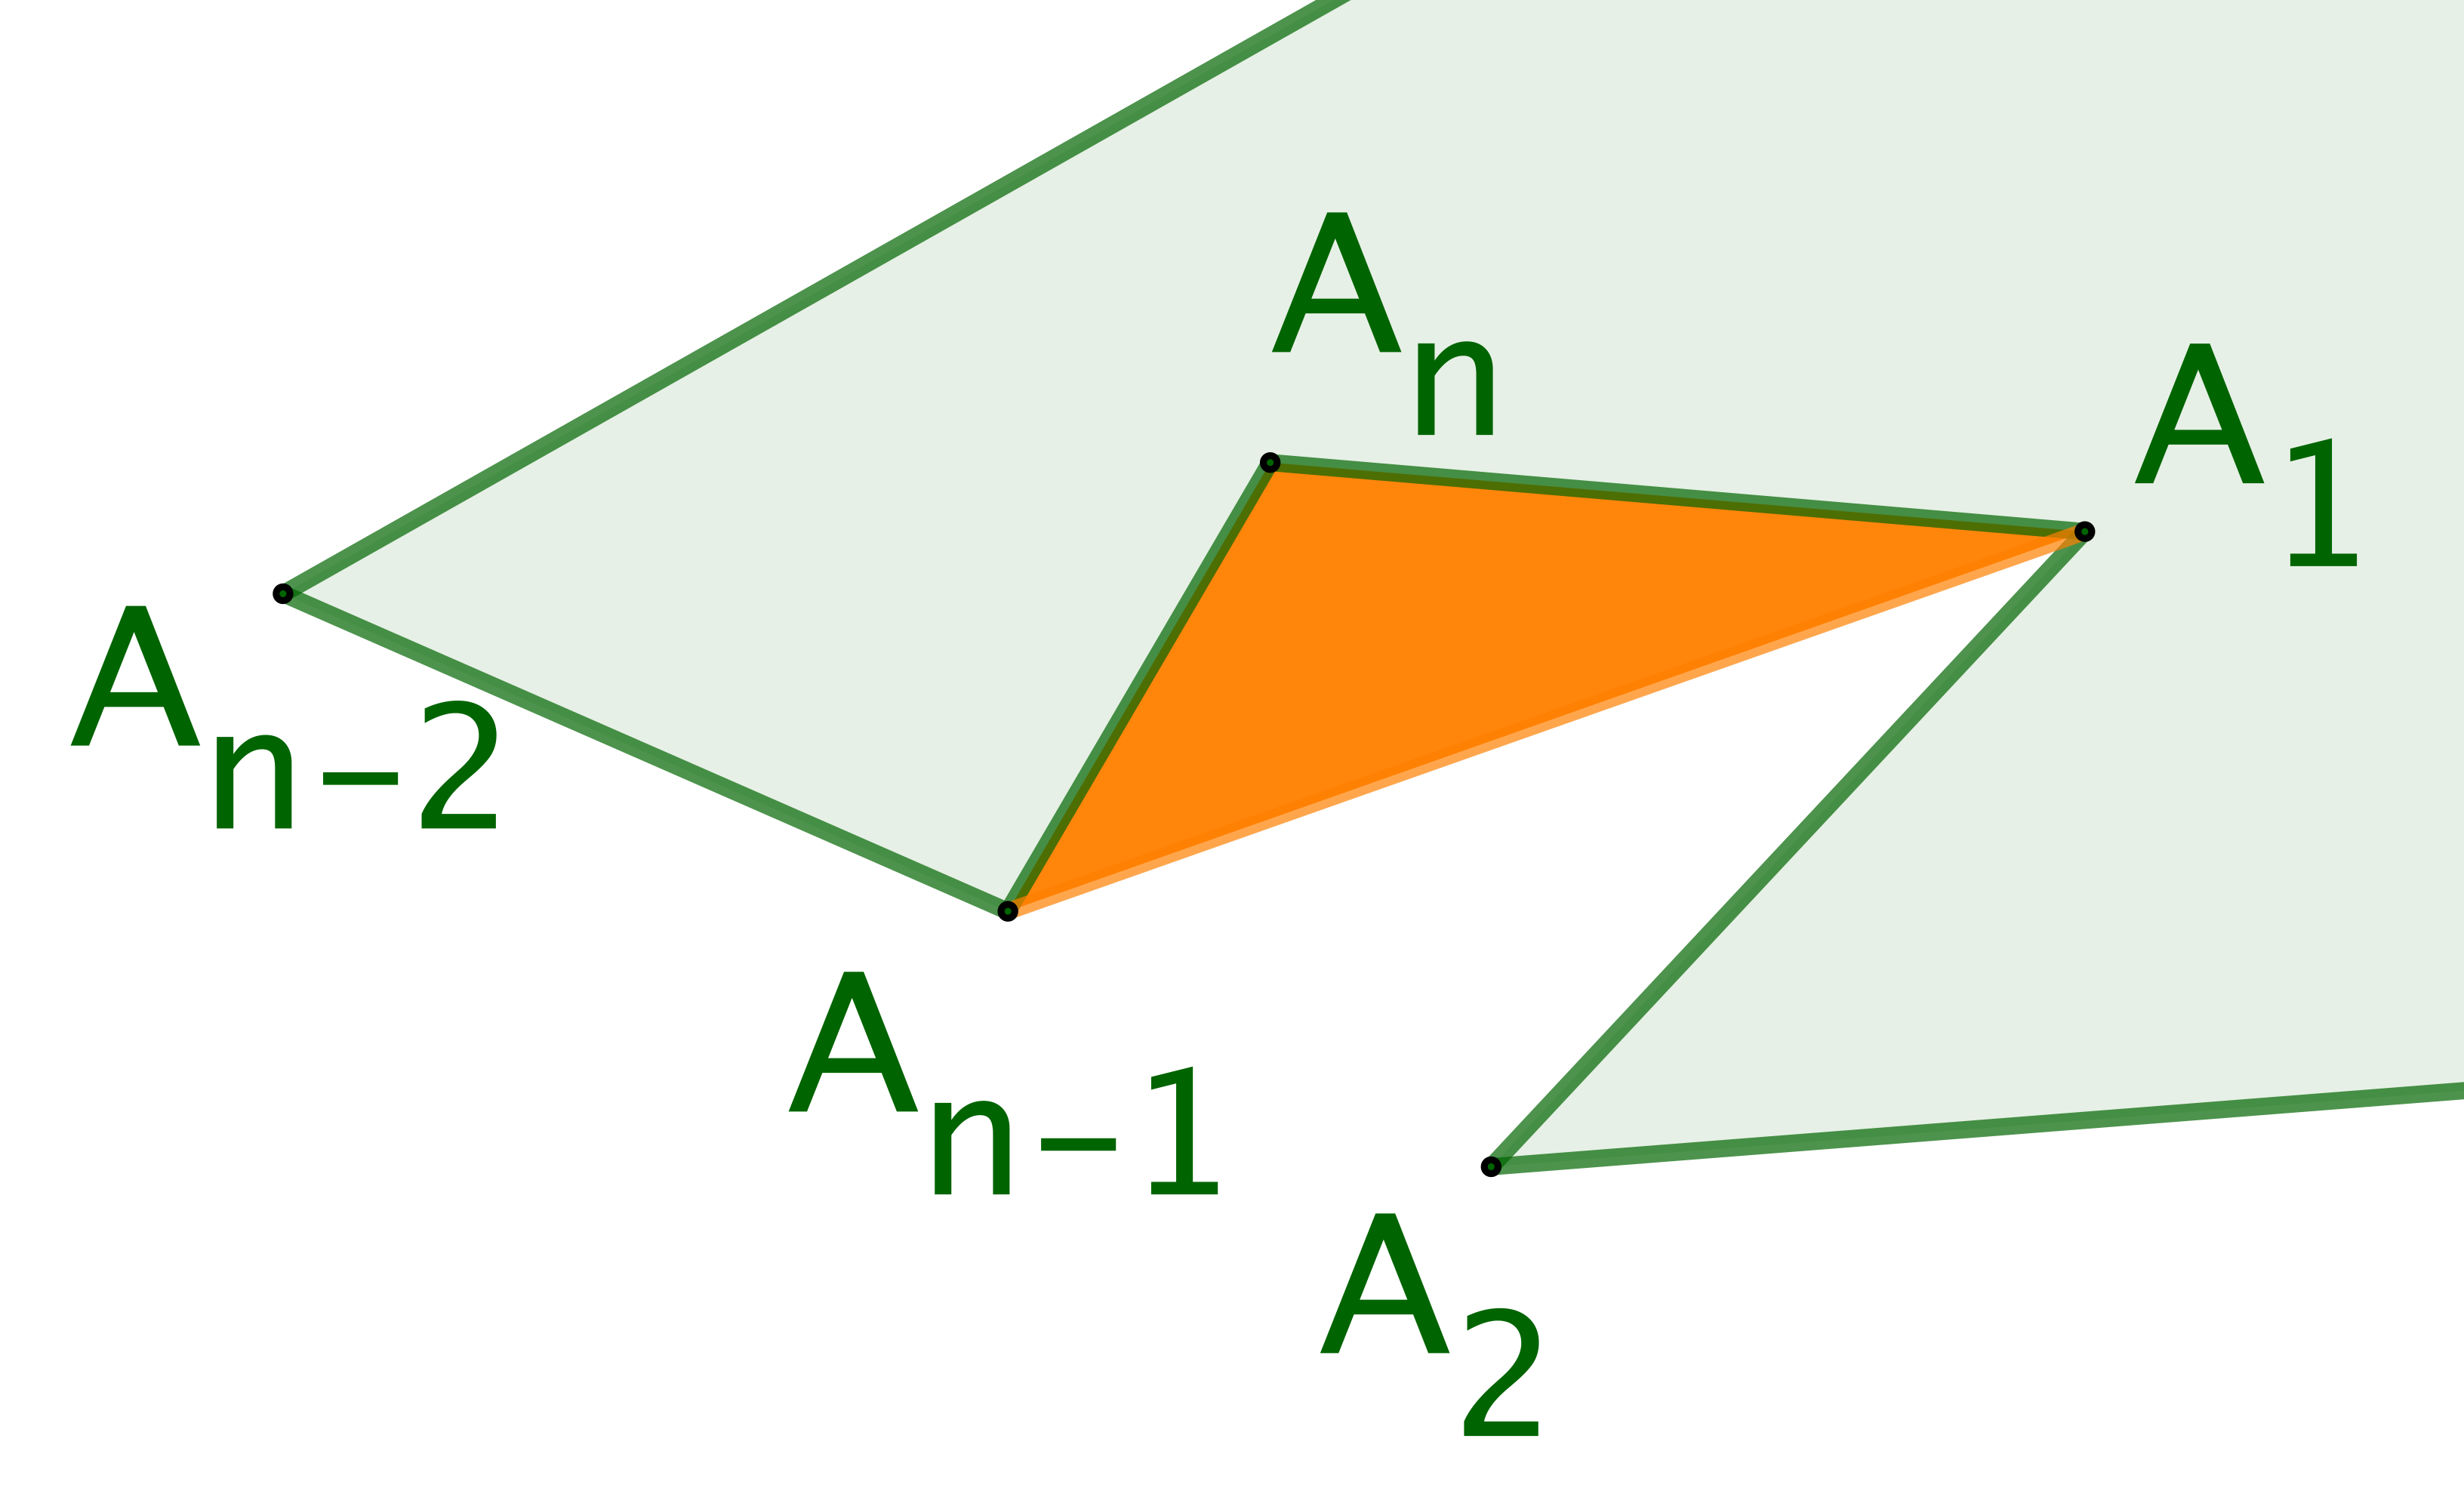
\includegraphics[scale=.4]{content/polygon/at-least-one/triangulation-proof-KO.png}
%
%        		\smallskip
%    	   		$A_{n-1} A_n A_1$ n'est pas une oreille.
%    		\end{center}
%    	\end{multicols}
%
%
%		\noindent
%		Posons $\setproba{P}^{\,\prime} = A_1 \cdots A_{n-1}$ où $k = n-1$ vérifie $k \in \NN_{\geq3}$. Par hypothèse, $\setproba{P}^{\,\prime}$ est positif. 
%		Nous arrivons finalement aux calculs élémentaires suivants en utilisant $A_1$ comme point de calcul de $\mu(\setproba{P})$.
%
%		\leavevmode\kern-2em%
%		\begin{stepcalc}[style=ar*]
%			\mu(\setproba{P})
%		%
%%		\explnext{}
%%			\dsum_{j=1}^{n} \det \big( \vect{A_1 A^{\,\prime}_j} , \vect{A_1 A^{\,\prime}_{j + 1}} \big)
%%		%
%		\explnext{}
%			\dsum_{j=1}^{n} \det \big( \vect{A_1 A^{\,\prime}_j} , \vect{A_1 A^{\,\prime}_{j + 1}} \big)
%%			+
%%			\det \big( \vect{A_1 A^{\,\prime}_n} , \vect{A_1 A^{\,\prime}_{n+1}} \big)
%		%
%		\explnext*{$A^{\,\prime}_{n+1} = A_1$ \\
%		           $A^{\,\prime}_i = A_i$ pour $i \leq n$}%
%		          {}
%			\dsum_{j=1}^{n-1} \det \big( \vect{A_1 A_j} , \vect{A_1 A_{j + 1}} \big)
%%			+
%%			\det \big( \vect{A_1 A_n} , \vect{A_1 A_1} \big)
%		%
%		\explnext{}
%			\dsum_{j=1}^{n-2} \det \big( \vect{A_1 A_j} , \vect{A_1 A_{j + 1}} \big)
%			+
%			\det \big( \vect{A_1 A_{n-1}} , \vect{A_1 A_n} \big)
%		%
%		\explnext*{Pour $\mu(\setproba{P}^{\,\prime})$, noter que 
%		        \\ $\det \big( \vect{A_1 A_{n-1}} , \vect{A_1 A_1} \big) = 0$.}{}
%			\mu(\setproba{P}^{\,\prime})
%			+
%			\mu(A_{n-1} A_n A_1)
%		\end{stepcalc}
%
%
%		\noindent
%		Par hypothèse de récurrence, nous savons que
%		$\mu(\setproba{P}^{\,\prime}) \geq 0$,
%		et comme $A_{n-1} A_n A_1$ est une oreille de $\setproba{P}$, la $3$-ligne $A_{n-1} A_n A_1$ est forcément positive, d'où $\mu(A_{n-1} A_n A_1) \geq 0$ d'après le cas de base.
%		Nous arrivons bien à $\mu(\setproba{P}) \geq 0$, ce qui permet de finir aisément la démonstration par récurrence.
%	\end{itemize}
%	
%	\null\vspace{-6ex}
%\end{proof}
%
%
%% ----------------------- %
%
%
%\begin{fact} \label{garea-ngone}
%    Pour tout \ngone\ $\setproba{P}$, nous avons:
%    $\area{\setproba{P}} = \frac12 \abs{\mu(\setproba{P})}$.
%\end{fact}
%
%
%\begin{proof}
%    Les deux points suivants permettent de faire une preuve par récurrence.
%
%    \begin{itemize}
%		\item \textbf{Cas de base.}
%		L'égalité est immédiate pour les triangles (c'est ce qui a motivé la définition de l'aire algébrique).
%
%
%		\item \textbf{Hérédité.}
%		Soit $\setproba{P} = A_1 \cdots A_n$ un \ngone\ avec $n \in \NN_{>3}$.
%		%
%		Comme $\mu(\setproba{P}^{\mathrm{op}}) = {} - \mu(\setproba{P})$ selon le fait \ref{nline-rota-inva}, nous pouvons choisir de parcourir $\setproba{P}$ positivement, puis de nous placer dans la situation de la démonstration du fait \ref{route-direction}:
%		$A_{n-1} A_n A_1$ est une oreille positive d'une triangulation à l'écoute du \ngone\ $\setproba{P}$, et $\setproba{P}^{\,\prime} = A_1 \cdots A_{n-1}$ un \kgone\ positif où $k = n-1$ vérifie $k \in \NN_{\geq3}$.
%		%
%		Nous arrivons finalement aux calculs élémentaires suivants.
%		
%		\leavevmode\kern-2em%
%		\begin{stepcalc}[style=ar*]
%			\area{\setproba{P}}
%		%
%		\explnext*{$A_{n-1} A_n A_1$ est une oreille de $\setproba{P}$.}%
%		          {}
%		    \area{\setproba{P}^{\,\prime}} + \area{A_{n-1} A_n A_1}
%		%
%		\explnext*{Hypothèse de récurrence et cas de base.}%
%		          {}
%		    \frac12 \abs{\mu(\setproba{P}^{\,\prime})} + \frac12 \abs{\mu(A_{n-1} A_n A_1)}
%		%
%		\explnext*{Voir le fait \ref{route-direction}.}%
%		          {}
%		    \frac12 \big( \mu(\setproba{P}^{\,\prime}) + \mu(A_{n-1} A_n A_1) \big)
%		%
%		\explnext*{Comme dans la preuve du fait \ref{route-direction}.}%
%		          {}
%		    \frac12 \mu(\setproba{P})
%		%
%		\explnext*{Voir le fait \ref{route-direction}.}%
%		          {}
%		    \frac12 \abs{\mu(\setproba{P})}
%		\end{stepcalc}
%    \end{itemize}
%    
%    \null\vspace{-3.5ex}
%\end{proof}
%
%
%
%
%
%
%
%
%
%
%
%
%
%
%% ----------------------- %
%





%\newpage % TEMP
%
%
%\begin{fact} \label{garea-cont}
%    Soit $n \in \NN_{\geq3}$ un naturel fixé.
%   
%   
%   le plan d'un repère orthonormé direct $\pvaxes{O | i | j}$
%   
%   
%    $\alpha: \setproba{U} \rightarrow \RRp$ qui à un uplet de $\setproba{U}$ associe l'aire généralisée du \ncycle\ qu'il représente.
%        Cette fonction est continue d'après le fait \ref{garea-cont}.
%\end{fact}
%
%
%\begin{proof}
%	GGGGG
%	
%	
%	pour les raisons suivantes où $\setproba{L} = A_1 A_2 \cdots A_n$ désigne un \ncycle.
%        %
%    \begin{itemize}
%        \item $\garea{\setproba{L}} = \dsum_{i} \area{\setproba{P}_i}$ où $\dcup_{i} \setproba{P}_i$ est frontière de la surface impaire de $\setproba{L}$.
%
%
%		\item Si $\dcup_{i} \setproba{P}_i = \emptyset$, alors $\garea{\setproba{L}} = 0$.
%
%
%		\item Si $\dcup_{i} \setproba{P}_i \neq \emptyset$, 
%		en posant $\setproba{P}_i = A_{i,1} A_{i,2} \cdots A_{i,n_i}$, 
%		le fait \ref{garea-ngone} nous permet d'écrire, en calculant les aires algébriques via l'origine $O$ du repère,
%		$ \garea{\setproba{L}} 
%		= \frac12 \dsum_{i} \big\lvert
%			\dsum_{k=1}^{n_i} \big( 
%				  x(A^{\,\prime}_{i,k}) y(A^{\,\prime}_{i,k+1}) 
%				- y(A^{\,\prime}_{i,k}) x(A^{\,\prime}_{i,k+1})
%			\big)
%		 \big\rvert$
%		.
%
%		\item XXXXX
%
%		\item XXXXX
%
%		\item XXXXX
%
%		\item XXXXX
%    \end{itemize}
%
%	\null\vspace{-6ex}
%\end{proof}
%
%
%% ----------------------- %
%
%
%\begin{fact} \label{suff-cond-ncycle}
%    Soit $n \in \NN_{\geq3}$ un naturel fixé.
%    Parmi tous les \ncycles\ de longueur fixée, non nulle, il en existe au moins un d'aire généralisée maximale, un tel \ncycle\ devant être a minima un \ngone\ convexe.
%\end{fact}
%
%
%\begin{proof}
%	Notons $\ell$ la longueur fixée.
%	%
%    \begin{itemize}
%        \item Munissant le plan d'un repère orthonormé direct $\pvaxes{O | i | j}$, on note $\setproba{Z}$ l'ensemble des \ncycles\ $\setproba{L} = A_1 A_2 \cdots A_n$ tels que
%        $\perim{\setproba{L}} = \ell$
%        et
%        $A_1\coord{0 | 0}$,%
%        \footnote{
%        	Le mot \og \emph{Zeile} \fg\ est une traduction possible de \og \emph{ligne} \fg\ en allemand.
%        }
%        puis $\setproba{U} \subset \RR^{2n}$ l'ensemble des uplets de coordonnées $\big( x(A_1) ; y(A_1) ; \dots ; x(A_n) ; y(A_n) \big)$ pour $A_1 A_2 \cdots A_n \in \setproba{Z}$.
%
%
%        \item $\setproba{U}$ est clairement fermé dans $\RR^{2n}$.%
%        \footnote{
%        	Il est faux d'affirmer que l'ensemble des \ngones\ est fermé: penser par exemple à un \ngone\ dont tous les sommets seraient fixés sauf un que l'on ferait d'entre vers l'un de ses voisins: ceci fait passer d'un \ngone\ à \kgone\ avec $k \leq n-1$.
%	        On peut aussi penser à des \ngones\ que l'on ferait tendre, en les \og aplatissant \fg, vers un \ncycle\ totalement \og plat \fg.
%        }
%        De plus, il est borné, comme le sont les coordonnées des sommets des \ncycles\ $\setproba{L}$ considérés (cf. la contrainte $\perim{\setproba{L}} = \ell$).
%        En résumé, nous savons que $\setproba{U}$ est un compact de $\RR^{2n}$.
%
%
%        \item Nous définissons la fonction $\alpha: \setproba{U} \rightarrow \RRp$ qui à un uplet de $\setproba{U}$ associe l'aire généralisée du \ncycle\ qu'il représente.
%        Cette fonction est continue d'après le fait \ref{garea-cont}.
%
%
%        \item Finalement, par continuité et compacité, $\alpha$ admet un maximum sur $\setproba{U}$.
%        Or, un tel maximum ne peut être atteint qu'en un \ngone\ convexe, au moins, selon le fait \ref{max-is-nconv}.
%    \end{itemize}
%    
%    \null\vspace{-6ex}
%\end{proof}
%
%
%% ----------------------- %
%
%
%\begin{fact} \label{suff-cond}
%    Soit $n \in \NN_{\geq3}$ un naturel fixé.
%    Parmi tous les \ngones\ de périmètre fixé, il en existe au moins un d'aire maximale, un tel \ngone\ devant être a minima convexe.
%\end{fact}
%
%
%\begin{proof}
%    Il suffit de convier les faits \ref{garea-ncycle}, \ref{garea-ngone} et \ref{suff-cond-ncycle} au même banquet des idées.
%\end{proof}
